\chapter{Comparaisons d'algorithmes}
\label{chap:resultats_comparaisons}


\section{Les méthodes pratiques} 
\label{sec:methodes_pratiques}
Nous cherchons maintenant à déterminer les performances et les qualités des différents algorithmes de proteus.
Pour évaluer les qualités des différents algorithmes de proteus, nous effectuons un ensemble de tests. 
Plusieurs questions se présentent alors,premièrement grâce à l' algorithme de type toulbar2 il est possible d'obtenir la séquence/conformation qui possède l'énergie de dépliement la plus haute. Cela constitue une information important qui va nous servir de point de comparaison. Mais le facteur temps pose problème, nous ne savons pas à l'avance quand toulbar2 termine. Et il apparaît d'emblée illusoire d'espérer voir toulbar2 converger dans toutes les situations qui nous intéressent dans un temps raisonnable, en particulier pour une situation où  toutes les positions du  backbone sont autorisé à muter et pour chaque type d'acide aminé la chaîne latérale peut prendre toutes les positions précédemment calculées dans la matrice. 


Dans la suite on appelle position active, une position pour laquelle, lors de la recherche par proteus, tous les types d'acides aminés sont autorisés et tous les rotamères de chaque type d'acide aminé sont autorisés.


\subsection{les protéines}
 
Les tests sont effectués sur neuf protéines choisies pour avoir des longueurs de backbone variés , plusieurs familles SCOP(?) représentées, mais aussi plusieurs structures pour chaque famille présente. Ainsi l'ensemble se décompose en deux protéines SH3 de 56 et 57 résidus, de trois protéines PDZ de longueur comprise entre 82 et 97 résidus  et enfin de trois protéines SH2  longues de 105 ou 109 résidus (Table~\ref{tab:protéines}).  


    \begin{table}[!htbp]
      \centering

      \begin{tabular}{cccc}

        \toprule
        Code PDB & résidus & nombre de positions & famille\\
        \cmidrule{1-4}
        1ABO & 	64-119	 & 	56	 & SH3 \\
        1CKA & 	134-190	 & 	57	 & SH3 \\
        1R6J & 	192-273	 & 	82	 & PDZ \\
        1G9O & 	9-99	 & 	91	 & PDZ \\
        2BYG & 	186-282	 & 	97	 & PDZ \\
        1BM2 & 	55-152	 & 	98	 & SH2 \\
        1O4C & 	1-105	 & 	105	 & SH2 \\
        1M61 & 	4-112	 & 	109	 & SH2 \\
        1A81 & 	9-117	 & 	109	 & SH2 \\
        \bottomrule

      \end{tabular}      
      \caption{Les protéines}
\label{tab:protéines}      
    \end{table}

\subsection{Description des tests}
\label{sec:description_tests}
Les tests sont réparties en deux ensembles:
\begin{enumerate}
\item un ensemble de tests où toutes les positions du backbone sont actives (cela correspond aux situations de design complet de protéines) 
\item un ensemble de tests où le nombre de positions actives est gardé sous contrôle .De façon à maîtriser la taille de l'espace d'exploration
\end{enumerate}


\paragraph{Ensemble 'Tout actif'}
\label{methode_TTactif}
Pour le premier ensemble de tests,La totalité de la matrice d'énergie est exploitée et pour chaque position l'espace d'exploration correspond à l'espace d'état déclaré dans le fichier .bb.C'est-à-dire que tous les types de résidu et tout les rotamères sont possibles à chaque position.
Comme l'espace des séquences/confirmations à explorer est gigantesque, nous ne faisons pas de tentative de recherche du GMEC  par méthode exacte. 

Nous effectuons des recherches avec les algorithmes suivants:

\begin{itemize}
\item heuristique  (noté H par la suite) ;
\item Monte-Carlo (noté MC);
\item ``'Replica Exchange'' (RE);
\end{itemize}


\paragraph{L'ensemble 'Nombre d'actifs limité'}

L'ensemble ``Nombre d'actifs limité''' est composé de six groupes de tests avec un nombre de positions actives fixe:  


\begin{enumerate}
\item aucune position active
\item une position active 
\item cinq positions 
\item dix  positions 
\item vingt positions 
\item trente positions 
\end{enumerate}

Lorsqu'une position n'est pas active, on fixe l'acide aminé de la position en utilisant l'acide aminé de la séquence native.

Le groupe `aucune position active ` est constitué d'un test par algorithme pour chaque protéine. Il y a donc neuf tests par algorithme.
Ce sont les tests pendant lesquels  la séquence d'acides aminés est fixe et correspond à la séquence native de la protéine.

Pour les tests avec une seule position active, comme des temps de calcul le permettent, nous décidons d'être exhaustif:
Toutes les positions sont testées, Il y a alors huit cent quatre tests par algorithme.
Pour tous les autres groupes de tests (5,10,20 et 30 positions actives) cinq tests sont effectués par protéine, c'est-à-dire quarante-cinq tests par algorithme.

\paragraph{le choix des positions actives}

Pour définir complètement les tests ,il reste maintenant à décrire comment le choix des positions actives pour les groupes numéro trois à numéro six a été effectué.
Il y a peu d'intérêt à tester des situations avec position active sans interaction avec les autres positions actives. 
En effet s'il existe une position active P dont chaque résidu est sans interaction avec tous les résidus possibles des autres positions actives, déterminer le meilleur état pour P est proche du test du groupe 2 avec P comme position active. Notons qu'en même que cela n'est pas exactement la même question parce que les positions actives différentes de P peuvent influencer la position de la chaîne latérale de positions inactives qui à leur tour peuvent influencer l'état de P.
Ainsi le choix des positions actives se fait non pas pas tirage aléatoire, car le risque d'avoir les positions peu en inter action est trop grand. Il se fait sous contrainte d'interaction.

\paragraph{positions en interactions}
Pour cela nous utilisons la notion de voisinage incluse dans proteus: 
Deux positions P et Q sont en interaction s'il existe un rotamère $r_P$ de P et un rotamère $r_Q$ de Q tels que:
\begin{displaymath}
 | E(r_P,r_Q) | > S_{Vois}
\end{displaymath} 
avec $S_{Vois}$ un seuil donné par utilisateur à la configuration de proteus (voir chap. ?? pour les détails).

Définissons maintenant la notion de n-uplet en interaction par la donnée de n positions avec $n \in \{5,10,20,30\}$ et d'un seuil  $S_{Vois}$  tels que pour toute paire de positions (P,Q) du n-uplet, P et Q sont en interaction.
\paragraph{}
Pour déterminer les positions actives,nous exécutons proteus en mode verbeux sans effectué d'optimisation.
Il existe plusieurs façons de procéder ,ici nous utilisons le mode Monte-Carlo avec une trajectoire de zéro pas. Ces exécutions produisent en sortie standard la liste des voisins pour chaque position au seuil donnée en paramètre.
Pour chaque protéine, nous exécutons proteus avec  $S_{Vois}$ égal à dix , cinq et un à tour de rôle. Nous obtenons quatre listes de voisins. 
Ensuite, nous cherchons dans les listes, par un script dédié, les n-uplets en interaction en partant de la liste de voisins au sens le plus fort, c'est-à-dire 10, vers la liste de voisins au sens le plus faible ($0.1$).La recherche s'arrête si cinq n-uplets sont trouvés.

Nous obtenons quarante cinq n-uplets pour le groupe à cinq (respectivement dix, vingt et trente ) positions actives pour un $S_{Vois}$ égale à dix (respectivement dix, un et un) (voir le détails en annexe~\ref{chap:annexe}). Chaque n-uplet nous créons un fichier de configuration de proteus dans lequel la balise <Space\_Constraints> fixe les positions restantes au type d'acide aminé présent dans la séquence native. 


\subsubsection{Définition de protocole comparable}

Nous voulons comparer les algorithmes très différents. Un algorithme peut garantir l'obtention du minimum global en énergie (GMEC) s'il termine, mais ne garantit pas qu'il termine, un autre permet un contrôle très fin du temps d'exécution sans garantie du GMEC, et d'autres enfin ont des objectifs plus ambitieux  qu'uniquement l'obtention du GMEC.
Mais le GMEC reste le meilleur point de commun. Nous allons donc y concentrer les comparaisons.

Nous devons noter également que l'obtention du GMEC est théorique, en pratique nous n'avons pas de preuve que le code de l'algorithme exact que nous utilisons soit sans bogue. Cependant,nous mettons de côté cette éventualité et dans toute la suite GMEC désigne aussi bien le minimum global en énergie que le résultat de toulbar2 lorsqu'il termine.  
\subparagraph{}
Le Monte-Carlo et le ``'Replica exchange'' possèdent de nombreux paramètres de configuration, ce qui rend l'ensemble des protocoles possibles très grand. Se pose alors la question de l'optimisation du protocole. L'objectif que nous nous fixons ici,n'est pas de recherche un protocole optimum pour chacun des tests, mais de tester un protocole optimisé par algorithme.
Nous allons alors dans un premier temps , recherche les meilleurs protocoles Monte-Carlo et les meilleurs protocoles ``'Replica Exchange'' sur l'ensemble de tests ``tout actifs''
Puis, sur la base des résultats obtenue, nous ferons l'ensemble des tests à positions actives limitées avec les meilleurs protocoles.
Le programme toulbar2 possède aussi de nombreuses options. Deux paramétrages différents seront utilisés.


Pour rendre les protocoles comparables, le temps d'exécution maximum est fixé à vingt-quatre heures, sauf mention contraire.
Toulbar2 donne sa meilleure séquence/conformation en dernier, il n'y a donc pas post-traitement nécessaire.
C'est également le cas pour le MC à condition de configurer l'impression de la trajectoire avec la balise $Print\_Threshold=0$. dans le fichier de configuration.
Pour le RE et l'Heuristique, un tri des séquences selon l'énergie est nécessaire. Mais il n'y a pas beaucoup de séquences: 
\begin{enumerate}
\item L' Heuristique fournit une séquence/conformation à chaque cycle.
\item Le RE avec $Print\_Threshold=0$ produit autant de fichiers de séquences/rotamères que de marcheurs.Chacun ne contenant pas plus de quelques dizaines de séquences/rotamères. 
\end{enumerate}

Nous pouvons donc négliger la durée du tri dans le temps total d'exécution.    


\subsection{Protocole Heuristique}

Pour l'algorithme Heuristique, il n'y a dans notre situation qu'un seul paramètre à renseigner: le nombre de cycles à effectuer. Quelques essais préliminaires sur la plus grosse protéine (Table~\ref{tab:protéines}) dans le cas où tout actif , montre que la version utilisée de proteus peut effectuer jusqu'à environ 110000 cycles sur nos machines de calculs en l'espace de vingt-quatre heures. Ainsi le protocole H est défini comme le protocole qui utilise le mode heuristique de proteus et qui effectue cent dix mille cycles. Nous définissons également les variantes H- , H+ et H++ comme des protocoles plus courts ou plus longs à facteur entier près (Table~\ref{tab:protoH}). Par ailleurs certains comparaisons de l'heuristique avec la MC ont été faites avec une version précédente de proteus notons h ce protocole. il diffère  aussi de H par le fait que les options d'optimisation du compilateur Intel -O2 contre -O3 pour H.    


    \begin{table}[!htbp]
      \centering

      \begin{tabular}{lr}

        \toprule
        Nom & nombre de cycles \\
        \cmidrule{1-2}
        H   & 110000 \\  
        H-  & 1100   \\  
        H+  & 330000 \\  
        H++ & 990000 \\  
        h   & 100000 \\  
        \bottomrule

      \end{tabular}      
      \caption{Les protocoles Heuristique}
\label{tab:protoH}      
    \end{table}

   \subsection{Protocoles Monte-Carlo}
\label{sec:MC}
On distingue deux ensembles de protocoles, Le premier où les noms  sont de la forme mc*, rassemble les protocoles utilisés pendant l'optimisation du Monte-Carlo.Le second est constitué du protocole retenue comme optimisé , plus une variante.     

\subsubsection{Paramétrage}

Les éléments à paramétrer pour l'algorithme Monte-Carlo sont les suivants:

\begin{enumerate}
\item la température
\item le nombre de pas (avec le nombre de trajectoires et la longueur de trajectoire )
\item Le seuil de voisinage
\item Les probabilités de changements de la séquences/rotamère
\end{enumerate}

Ce qui représente un ensemble de protocoles trop grand pour une approche exhaustive. Nous allons faire varier les paramètres un par un.

La température est le paramètre principale du Monte-carlo, c'est lui qui contrôle le taux d'acceptation du critère de Metropolis.Alors la première étape de cette optimisation va consisté à faire variés la température , entre 0.001 et 0.5 , en conservant les autres paramètres fixés (protocoles de mc0 à mc5).Le nombre de pas total effectué est le produit de deux paramètres, le nombre de trajectoires et la longueur de trajectoire. les protocoles mc1b et mc2b testent l'effet d'une augmentation du nombre de pas. Tandis que mc2d teste l'effet de variation du rapport nombre de trajectoire sur la longueur.
Le protocole mc2e s'intéresse aux probabilités de changement de la trajectoire. Il y a cinq balises dans proteus qui contrôle ces changements:

\begin{description}
\item[<Prot>] donne la probabilités de modifications de  rotamère à une postions.
\item[<Prot\_Prot>] donne la probabilités de modifications de  rotamère à deux positions.
\item[<Mut>] donne la probabilités de modifications de type de résidu à une position.
\item[<Mut\_Prot>] donne la probabilités de modifications de  rotamères à deux positions.
\item[<Mut\_Mut>] donne la probabilités de modifications de type de résidu à deux positions.
\end{description}

La table~\ref{tab:protoMC} donne les probabilités utilisées par ces cinq paramètres dans l'ordre de la liste précédente. 

 Enfin mc4b se distingue des autres par un seuil de voisinage plus grand ((Table~\ref{tab:protoMC})).


\paragraph{Second version de proteus}
Pour l'étape suivante, qui consiste à la comparaison avec les autres algorithmes, quatre protocoles sont utilisés. Les protocole MCa et MCb s'inspirent fortement de mc2d et mc2e , en étant adapté à la contrainte du temps de calculs de la comparaison d'algorithmes et un utilisant la nouvelle version de proteus (les lettres capitales dans le nom des protocoles signifie l'utilisation de la dernière version de proteus,ceci dans toute la suite). MCa- est une de MCa avec une trajectoire six fois plus courte.Enfin, MC0 s'inspire de mc0 dans le sens où la température est suffisamment froide pour que nous puissions considérer qu'il n'y a pas de baisse de l'énergie au court d'une trajectoire.
  

    \begin{table}[!htbp]
      \centering

      \begin{tabular}{llrrcc}

        \toprule
        Nom & Temp & Long. de trajectoire(mega) & Nb de trajectoires  & Voisin & Proba \\
        \cmidrule{1-6}
        mc0   & 0.001 &  3  &  1000  & 10 & 0; 1; 0.1; 0 ;0 \\      
        mc1   & 0.1   &  3  &  1000  & 10 & 0; 1; 0.1; 0 ;0 \\  
        mc2   & 0.2   &  3  &  1000  & 10 & 0; 1; 0.1; 0 ;0 \\ 
        mc3   & 0.3   &  3  &  1000  & 10 & 0; 1; 0.1; 0 ;0 \\               
        mc4   & 0.5   &  3  &  1000  & 10 & 0; 1; 0.1; 0 ;0 \\  
        mc5   & 0.7   &  3  &  1000  & 10 & 0; 1; 0.1; 0 ;0 \\  
        mc1b  & 0.1   &  6  &  1000  & 10 & 1; 1;   1; 1 ;0 \\  
        mc2b  & 0.2   &  6  &  1000  & 10 & 0; 1; 0.1; 0 ;0 \\      
        mc2c  & 0.2   &  3  & 10000  & 10 & 0; 1; 0.1; 0 ;0 \\   
        mc2d  & 0.2   &  3000  &  1 & 10  & 0; 1; 0.1; 0 ;0 \\ 
        mc2e  & 0.2   &  3  &  1000  & 10 & 1; 0; 0.1; 0 ;0 \\     
        mc4b  & 0.5   & 10  &   100  & 10 & 0; 1;   0; 1 ;0 \\
        \cmidrule{1-6}
        MC0   & 0.001 &  1000  &  1  & 10 & 1; 0; 0.1; 0 ;0 \\            
        MCa   & 0.2   &  6000  &  1  & 10 & 1; 0; 0.1; 0 ;0 \\   
        MCa-  & 0.2   &  1000  &  1  & 10 & 1; 0; 0.1; 0 ;0 \\   
        MCb   & 0.2   &  6000  &  1  & 10 & 0; 1; 0.1; 0 ;0 \\      


        \bottomrule   

        
      \end{tabular}      
      \caption{Les protocoles Monte-Carlo}
\label{tab:protoMC}      
    \end{table}

   \subsection{Les protocoles Replica Exchange} 

L'algorithme ``Replica Exchange'' (RE) est une extension du Monte-Carlo , Les paramètres d'un protocole RE sont ceux d'un protocole Monte-Carlo plus d'autres paramètres:

\begin{itemize}
\item le nombre de marcheurs
\item la température pour chaque marcheur
\item la période de ``swap'', c'est-à-dire la période  (en nombre de pas) à  laquelle le test de Hasting sur l'échange de température et éventuellement l'échange ,sont effectués.
\end{itemize}
Pour avoir des exécutions en parallèle sans plusieurs marcheurs  par coeur du processeur, nous limiter nos tests à quatre ou huit marcheurs.
La distribution des températures est un éléments déterminant dans le comportement des marcheurs, car c'est elle qui pilote en grande partie le taux d'acceptation des échanges de températures. Nous suivant l'idée proposée par Kofke de lui faire suivre une progression géométrique ( $ \frac{T_i}{T_{i+1}}=C $ , avec C une constante)~\citep{refRE1,refRE2,refRE3}. Ceci garantie alors que le taux d'acceptation d'échange entre $T_i et T_{i+1}$ soit égale pour tout nos i.De plus nous souhaitons centrer à peu près, nos distributions sur la température ambiante.

Voici les températures pour le RE quatre marcheurs:

\begin{itemize} 
\item 10, 1, 0.1 et 0.01
\item 2, 1, 0.5 et 0.25 
\item 1, 0.5, 0.25 et 0.125
\end{itemize} 

,et celles pour le RE huit marcheurs:

\begin{itemize} 
\item 3 , 2 , 1.333 , 0.888 , 0.592 , 0.395 , 0.263 et 0.175 
\item 10 , 3.16 , 1 , 0.316 , 0.1 , 0.0316 , 0.01 et 0.00316
\end{itemize} 

Ici les protocoles ne se font qu'avec une seule trajectoire par marcheur. Et la contrainte du temps de calculs se comprends comme vingt-quatre heures de calculs cumulées sur tous les marcheurs.
Ainsi les longueurs de trajectoire sont définit pour le RE quatre marcheurs comme le quart d'une trajectoire MC, pour le RE huit marcheurs comme le huitième.

La table~\ref{tab:protoRE} donne les probabilités utilisées par les cinq balises qui contrôlent les modifications de la séquence/conformation à chaque pas, dans l'ordre de la liste de la section~\ref{sec:MC}. 
    
    \begin{table}[!htbp]
      \centering

      \begin{tabular}{llrrrcc}

        \toprule
        Nom & marcheurs &Temp & Traj (mega)& seuil voisin  & Proba & swap period (mega)\\
        \cmidrule{1-7}
        RE4a   & 4 & 10<->0.01    &  1500 & 10 & 1; 0; 0.1; 0 ;0 &  7.5\\  
        RE4b   & 4 & 1<->0.125    &  1500 & 10 & 1; 0; 0.1; 0 ;0 &  7.5\\  
        RE4c   & 4 & 2<->0.25     &  1500 & 10 & 1; 0; 0.1; 0 ;0 &  7.5\\  
        RE8a1  & 8 & 10<->0.00316 &  750  & 0  & 1; 0; 0.1; 0 ;0 &  2.5\\  
        RE8a2  & 8 & 10<->0.00316 &  750  & 10 & 1; 0; 0.1; 0 ;0 &  2.5\\  
        RE8b1  & 8 & 3<->0.175    &  750  & 10 & 0; 1; 0.1; 0 ;0 &  7.5\\
        RE8b2  & 8 & 3<->0.175    &  750  & 10 & 1; 0; 0.1; 0 ;0 &  7.5\\
        RE8b3  & 8 & 3<->0.175    &  750  & 10 & 1; 0; 0.1; 0 ;0 &  1\\
        \bottomrule

      \end{tabular}      
      \caption{Les protocoles Replica Exchange}
\label{tab:protoRE}      
    \end{table}

   \subsection{Les protocoles Toulbar2} 


Après avoir convertit nos matrices au format wcsp grâce à un script dédié,nous pouvons utiliser toulbar2.
Le protocole toulbar2 de recherche du GMEC est le suivant:
Le binaire toulbar2 de version 0.9.7.0 est lancé avec les options -l=3 -m -d: -s, ce qui correspond au paramétrage conseillé dans la documentation CDP~\citep{reftoulbar1,reftoulbar2}. Si au bout de vingt-quatre heures l'exécution est terminée, le protocole est achevé. Sinon le programme est arrêté et une seconde version (la 0.9.6.0) est lancé avec les options -l=1 -dee=1 -m -d: -s. Au bout de vingt-quatre heures si le programme n'est pas terminée, il est arrêté. La dernière séquence/conformation imprimer en sortie est collectée. Le choix de la seconde version et du paramétrage fait suite à une discussion avec monsieur Seydou Traoré.  

Toulbar2 est également capable de fournir la listes des séquences/conformations dont l'énergie est comprise entre celle du GMEC, $E_{GMEC}$ et une autre $E_{upper\_bound}$ donnée en paramètre. Pour cette fonctionnalité nous utilisons le paramétrage:  -d: -a -s -ub=$E_{upper\_bound}$.

   \subsubsection{Superfamily/SCOP} 

Superfamily est un ensemble avec d'une base de données composée de modèle de Markov cachés~\citep{refSuperfamily}

\begin{itemize}
\item Une base de données de modèles de Markov cachés, où chaque modèle représente une structure 3D d'un domaine de la classification SCOP.
\item une série de script qui annote une séquence de protéine donnée en entrée à partir des informations de la base. Ici nous utilisons uniquement l'association au modèle 3D le plus vraisemblable. 
\end{itemize}

Nous travaillons avec la base de données à la version 1.75, et en conjonction, nous utilisons SAM (version 3.5)~\citep{refSam} et HMMER (version 3.0)~\citep{refHmmer} recommandée par l'équipe de Superfamily. Le paramétrage utilisé est celui par défaut.

\subsection{identité par position et par séquence}

\subsection{Taux d'identité}


\subsubsection{Taux d'identité de séquences}

Soient S et N deux séquences d'acides aminés de même longueur l.

Le Taux d'identité $Id(S,N)$ de S par rapport N est égal au pourcentage de position où l'acide aminé est identique dans S et N. C'est-à-dire

  $ Id(S,N) =\frac{\sum_{1<i<l} \mathds{1}(s_i,n_i)}{l} \times 100$ 

avec $s_i$ et $n_i$ l'acide animé en i de S et de N respectivement, et $\mathds{1}(x,y)$ la fonction qui vaut 1 lorsque x=y et 0 sinon. 

\subsubsection{Taux d'identité par position}

Nous définissons également un taux d'identité d'un alignement $A_S$  à la position i par rapport à une séquence N de même longueur comme:

$Id(A_{S},i) = \frac{\sum_{1<j<m} \mathds{1}(s_i^j,n_i)}{m} \times 100$ , avec m le nombre de séquences de $A_S$.

\subsection{Similarité}

Les taux d'identités qui viennent d'être présentés nous permettre de mesurer une ressemblance d'un séquence ou d'un ensemble de nos séquences produites par rapport à la séquence native. Mais cela n'est pas notre principale objectif.Et nous devons évaluer nos séquences par rapport à l'ensemble des séquences du domaine protéique de la séquence native.  

   \subsubsection{Alignements Pfam} 
La base de données Pfam (Protein families database)~\citep{refPfam} regroupe les domaines protéiques connus en famille. Chaque famille  étant représentées des alignements multiples de séquences et des profiles de modèles de Markov cachés~\citep{refPfam}. Dans la suite nous n'utiliserons l'alignement dit ``seed'' qui ne contient q'un petit ensemble de membres représentatifs de famille et l'alignement ``full'' qui est généré par modèle de Markov caché à partir de l'aligement ``seed''. Les alignements correspondent pour nous aux familles PF00017 (domaine SH2), PF00018  (domaine SH3) et PF00595 (domaine PDZ).

 \subsubsection{Score BLOSUM}

Pour tenir compte des ressemblances et des différences entre les acides aminés lors d'une substitution, nous avons besoin d'une matrice de coût.Nous utilisons la matrice BLOSUM62 (BLOcks SUbstitution Matrix)~\citep{refBLOSUM} qui est construite à partir de blocs l'alignement très conservées (ici plus de 62\% d'identités).Les fréquences des mutations y sont calculées.Le score BLOSUM d'une substitution est alors le logarithme de la fréquence de la mutation correspondante.À cela est ajouté un scrore de pénalités pour l'insertion d'un gap (c'est-à-dire un saut dans l'alignemnet).

On définit alors simplement un score de similarité de deux séquences de même longueur comme la somme des scores BLOSUM62 sur toutes les positions. De même le score de similarité d'un alignement par rapport à une séquence sera définit comme la moyenne des score de similarité sur ensemble des séquences de l'alignement. Et enfin une score de similarité de deux ensembles de séquences alignés entre eux comme la moyenne des scores de similarité du premier ensemble par rapport aux séquences du second.  

\subsection{similarité d'un ensemble à une famille Pfam}

Afin de calculer un score de similarité d'un ensemble de nos séquences par rapport à une famille Pfam, il faut commencer par aligner nos séquences avec l'alignement de la famille.Pour cela nous utilisons le programme d'alignement BLAST~\citep{refBLAST}.Il implémente une heuristique qui recherche puis étend les meilleurs alignement locaux. Nous procédons comme suit:
\begin{enumerate}
\item La commande blastpgp est utilisée avec comme database (paramètre -d ) l'alignement Pfam et comme séquence en entrée ( paramètre -i ) la séquence native. 
\item Dans la sortie blast, la séquence qui produit l'alignement le plus significatif avec la native est collectée, notons la $S_0$. 
\item L'alignement blast est alors utilisé pour positionner la native par rapport à $S_0$ et les gaps nécessaires pour aligner la native à $S_0$ sont ajoutés.
\item  Le positionnement et les gaps sont alors appliqués tels quels à la liste de nos séquences.

\end{enumerate}


\subsection{Réparition de l'energie selon les centiles }

Pour comparer différentes distributions d'ensemble de séquences/conformations selon l'énergie,nous déterminons les centiles de la façon suivante: 

\begin{enumerate}
\item l'ensemble de séquences/conformations est trié selon l'énergie.
\item L'intervalle entre la meilleur énergie et la moins bonne est divisé en cent intervalles consécutifs contenant le même nombre de séquences/conformations (un centième du cardinal de l'ensemble).
\item les quatre-vingts dix neufs valeurs d'energie obtenues par ce découpage sont les centiles.   
\end{enumerate}


\clearpage

    \section{Résultats} 

    \subsection{Paramétrage du protocole Monte-Carlo}

Le choix des paramètres du protocole Monte-Carlo est décidé sur des tests sur les sept protéines avec toutes les positions actives.


   \subsubsection{Température et meilleures énergies} 
Nous utilisons les protocoles de mc0 à mc5, voir table~\ref{tab:ener_mc} pour évaluer d'effet du paramètre température dans la recherche de séquences/rotamères de meilleurs énergies.La table~\ref{tab_ener_mc} présente les résultats obtenus arrondis à la Kcal/mol inférieure. L'énergie proteus est l'énergie de dépliement c'est-à-dire l'énergie qu'il faut fournir à la protéine pour la déplier.Donc les meilleurs dans la table (et dans toutes les autres tables ) sont les énergies les plus grandes. Les tests aux températures les plus froides (0.001 et 0.1) donnent les meilleurs résultats  pour la majorité des protéines. Cependant la dégradation des performances est lente avec l'augmentation des températures. Et les résultats pour les températures intermédiaires (0.2 et 0.3) sont souvent très proches des meilleurs résultats.    

    \begin{table}[!htbp]
      \centering


      \begin{tabular}{ccccccc}

     
        \toprule
         test & 0.001$^a$ & 0.1$^b$ & 0.2$^c$  & 0.3$^d$ & 0.5$^e$ & 0.7$^f$  \\
        \cmidrule{1-7}
        1ABO & -270 & -270 & -270 & -271 & -281  & -289 \\      
        1CKA & -251 & -247 & -252 & -252 & -261  & -267 \\  
        1BM2 & -482 & -486 & -483 & -486 & -516  & -541 \\  
        1M61 & -480 & -481 & -483 & -485 & -506  & -523 \\  
        1O4C & -532 & -527 & -533 & -536 & -563  & -590 \\  
        1G9O & -423 & -425 & -426 & -432 & -450  & -462 \\  
        1R6J & -411 & -411 & -412 & -417 & -435  & -449 \\  

        \bottomrule        
      \end{tabular}
      

      \caption{Meilleur énergie selon la température,($^a$ le protocole mc0,$^b$ mc1,$^c$  mc2,$^d$ mc3,$^e$ mc4,$^f$ mc5 )}    
      \label{tab:ener_mc}
    \end{table}
 
   \subsubsection{Température et taux d'identité de séquences} 
\label{sec:T_et_I}
Nous poursuivons la comparaison des protocole mc0-mc5 en regardant le taux d'identité entre les séquences d'acides aminés et la séquence native. Pour cela, nous reprenons les séquences/conformations obtenues et triées selon l'énergie décroissante. Nous sélectionnons dans cette liste, les dix mille premières séquence pour chaque test. Les résultats sont présentés table~\ref{tab:ident_mc}.Nous obtenons des taux d'identités globalement compris entre 20 et 40\% , avec le plus suivant des valeurs proches de 30\%. Les résultats à température 0.2 et 0.3, sont aussi bon que ceux à température 0.1 et légèrement meilleurs que pour 0.001. Ici aussi il y a une dégradation aux température les plus hautes, faible à 0.5, plus nette à 0.7.

    \begin{table}[!htbp]
      \centering

      \begin{tabular}{ccccccc}
      
        \toprule
         test & 0.001$^a$ & 0.1$^b$ & 0.2$^c$  & 0.3$^d$ & 0.5$^e$ & 0.7$^f$  \\
        \cmidrule{1-7}
        1ABO & 33 & 33 & 33 & 32 & 32  & 30 \\      
        1CKA & 26 & 27 & 27 & 27 & 26  & 26 \\  
        1BM2 & 26 & 27 & 27 & 28 & 25  & 23 \\  
        1M61 & 40 & 41 & 41 & 41 & 41  & 39 \\  
        1O4C & 21 & 21 & 21 & 21 & 20  & 19 \\  
        1G9O & 35 & 35 & 36 & 37 & 36  & 33 \\  
        1R6J & 33 & 33 & 32 & 32 & 31  & 29 \\  
        \bottomrule
        
      \end{tabular}
      

      \caption{Pourcentage d'identité de séquences selon la température,($^a$ le protocole mc0,$^b$ mc1,$^c$  mc2,$^d$ mc3,$^e$ mc4,$^f$ mc5 )}      
      \label{tab:ident_mc}
    \end{table}



   \subsubsection{Température et résultats Superfamily} 

Nous évaluons maintenant, la similarité que peuvent avoir nos séquences putatives avec la structure 3D du domaine de la protéine. Nous lancer Superfamily sur chaque ensemble de dix milles séquences (voir \ref{sec:T_et_I}). Le tableau \ref{tab:SF_mc} présente le nombre de séquences attribuées au domaine de la séquence native par cet outil. Les résultats sont bons, sauf pour les températures les plus chaudes, la grande majorité des séquences sont attribuées au domaine natif respectif (les domaines sur en Table~\ref{tab:protéines}).Ici, les deux températures intermédiaires font quasiment jeu égal avec les deux températures les plus froides.
    \begin{table}[!htbp]
      \centering
      
      \begin{tabular}{crrrrrr}      
        \toprule
         Protéine & 0.001$^a$ & 0.1$^b$ & 0.2$^c$  & 0.3$^d$ & 0.5$^e$ & 0.7$^f$  \\
        \cmidrule{1-7}
        1ABO & 7382  & 8374 & 6764 & 5033 & 2576  & 1255  \\      
        1CKA & 8045  & 8497 & 9139 & 9534 & 8060  & 2490  \\  
        1BM2 & 8073  & 8002 & 6861 & 7869 & 4458  & 2821  \\  
        1M61 & 9489  & 9662 & 9825 & 9777 & 9822  & 8744  \\  
        1O4C & 7124  & 7702 & 6909 & 7849 & 7623  & 4847  \\  
        1G9O & 10000 & 10000 & 10000 & 10000 & 10000  & 9942 \\  
        1R6J & 9878  & 9871 & 9796 & 8794 & 5387 & 3787 \\  

        \bottomrule
        
      \end{tabular}
      

      \caption{Résultats Superfamily pour les dix mille séquences de meilleur énergie selon la température,($^a$ le protocole mc0,$^b$ mc1,$^c$  mc2,$^d$ mc3,$^e$ mc4,$^f$ mc5 )}      
      \label{tab:SF_mc}
    \end{table}



   \subsubsection{Température et entropie} 

Il apparaît assez clairement, de part le principe du test de metropolis-Hasting, que le Monte-Carlo à basse température explore une partie de l'espace plus petite qu'au haute température. Il est alors légitime de mesurer cet effet sur les ensembles de dix milles séquences obtenues. Nous utilisons un alphabet A (voir table \ref{tab:Alphabet}) réduit à six classes d'acides aminés comme proposée dans~\citep{refAlphabet} qui permet de se focaliser sur les différences physico-chimiques des acides aminés.  

L'entropie par position $H_i$ est alors définit de la façon suivante.
Pour i une position dans la séquence, notons $f_{i}(a)$ la fréquence en i, de la lettre a de l'alphabet A . Alors 
$H_i=  - \sum_{a \in A} f_{i}(a) * log( f_{i}(a) ) $  

Puis, nous calculons la moyenne sur les postions des $exp(H_i)$ pour nos tests. Les résultats sont sur le tableau \ref{tab:Entro_mc}.


    \begin{table}[!htbp]
      \centering
      
      \begin{tabular}{ccccc}
        \toprule
        acide aminé & alphabet & & acide aminé & alphabet \\
        \cmidrule(r){1-2}   \cmidrule(r){4-5}     
        L & 1 & & S & 4 \\
        V & 1 & & T & 4 \\
        I & 1 & & P & 4 \\
        M & 1 & & E & 5 \\
        C & 1 & & D & 5 \\
        F & 2 & & N & 5 \\
        Y & 2 & & Q & 5 \\
        W & 2 & & K & 6 \\
        G & 3 & & R & 6 \\
        A & 4 & & H & 6 \\
        \bottomrule                
      \end{tabular}
      \caption{Alphabet réduit}      
      \label{tab:Alphabet}

    \end{table}

Nous observons la diminution systématique de l'entropie avec cette de la température. Cela représente une moindre diversité dans les séquences obtenues pour les températures des plus froides.

    \begin{table}[!htbp]
      \centering
      
      \begin{tabular}{lllll}
        \toprule
         Protéine & 0.001$^a$ & 0.1$^b$ & 0.2$^c$  & 0.3$^d$ \\
        \cmidrule{1-5}      
        1ABO & 1.68 & 1.80 & 1.84 & 2.14  \\  
        1CKA & 1.85 & 2.06 & 2.09 & 2.13  \\ 
        1BM2 & 1.88 & 1.94 & 1.96 & 2.11  \\ 
        1M61 & 1.53 & 1.60 & 1.62 & 1.79  \\ 
        1O4C & 2.18 & 2.21 & 2.23 & 2.3   \\ 
        1G9O & 1.64 & 1.68 & 1.84 & 2.07  \\ 
        1R6J & 1.75 & 1.79 & 1.94 & 2.20  \\ 
        \bottomrule               
      \end{tabular}
      \caption{Moyennes sur les positions des exp(entropies) pour les dix mille séquences de meilleur énergie,($^a$ le protocole mc0,$^b$ mc1,$^c$  mc2,$^d$ mc3)}      
      \label{tab:Entro_mc}
    \end{table}

   \subsubsection{Trajectoire et pourcentage d' identité} 

Le nombre de pas effectués dans les protocoles Monte-Carlo est le produit du nombre de trajectoires par le longueur de trajectoire. Nous comparons le pourcentage d'identité de séquences par rapport à la séquence native pour des protocoles ne variant que par le nombre de trajectoires ou la longueur de la trajectoire. Deux ensembles sont traités, mc1 et mc1b ( mc1 mais avec des trajectoires deux fois plus grandes) d'une part et mc2, mc2b , mc2c et mc2d d'autre part, avec mc2b ayant des trajectoire deux fois plus grandes de mc2, mc2c dix fois plus de trajectoire que mc2 et le même nombre de pas mais une seule trajectoire pour mc2d par rapport mc2.
Les résultats sont visibles à la table \ref{tab:Traj_ident}.L'effet du doublement de la longueur de la trajectoire existe mais est très faible. De même l'augmentation du nombre de trajectoires, pourtant drastique, n'apporte quasiment rien. Élément intéressant, à nombre de pas identique, il n'y pas de différence notable entre le protocole mille trajectoires et celui à une seule.  

    \begin{table}[!htbp]
      \centering
      
      \begin{tabular}{ccccccc}

        \toprule
        Protéine & mc1 & mc1b & mc2  & mc2b & mc2c & mc2d  \\
        \cmidrule{1-7}      
        1ABO & 33 & 33 & 33 & 33 & 33  & 33 \\      
        1CKA & 24 & 25 & 25 & 26 & 25  & 25 \\  
        1BM2 & 26 & 27 & 27 & 27 & 27  & 27 \\  
        1M61 & 40 & 40 & 41 & 42 & 41  & 41 \\  
        1O4C & 21 & 21 & 21 & 21 & 21  & 21 \\  
        1G9O & 35 & 35 & 36 & 36 & 36  & 36 \\  
        1R6J & 33 & 33 & 32 & 32 & 33  & 33 \\  
        \bottomrule
      \end{tabular}
      

      \caption{Pourcentage d'identité en variant la longueur et le nombre de trajectoires.}      
      \label{tab:Traj_ident}
    \end{table}


   \subsubsection{Mutations et pourcentage d' identité} 
Jusqu'à présent nous avons utilisé le même mode de modification de la séquence/conformation entre chaque pas Monte-Carlo pour tous les protocoles. Il s'agît du mode qui utilise les balises <Prot\_Prot> avec une valeur à 1 et <Mut> avec une valeur à 0.1. Cela veut dire qu'à chaque pas deux rotamères sont modifiés sans changement du type de résidu et qu'une troisième position change d'acide aminé avec une probabilité de 0.1. Nous allons comparer ce mode de modification (avec les protocoles mc1 et mc2 ) avec un mode où seulement  le rotamère est changé à une position sans changement de type et une seconde position change d'acide aminé la même probabilité que précédemment, 0.1 (avec les protocoles mc1b et mc2e). Les résultats sont visibles à la table ((Table~\ref{tab:mut_ident})). Nous voyons que le en ce qui concerne le premier couple de protocole, il n'y a un déclin pour tous les tests. Pour le second il y a également une dégradation des performances globales mais elle n'est pas systématique. Il y a même une amélioration pour la protéine 1R6J.  


    \begin{table}[!htbp]
      \centering
      
      \begin{tabular}{ccccc}      
          \toprule
          Protéine & mc1 & mc1b & mc2 & mc2e \\
          \cmidrule{1-3}
          
          1ABO & 33 & 30 & 33 & 32 \\      
          1CKA & 27 & 24 & 27 & 26 \\
          1BM2 & 27 & 22 & 27 & 27 \\
          1M61 & 41 & 35 & 41 & 41 \\
          1O4C & 21 & 18 & 21 & 20 \\
          1G9O & 35 & 31 & 36 & 29 \\
          1R6J & 33 & 27 & 32 & 33 \\ 
          \bottomrule
          
        \end{tabular}
        
        \caption{Pourcentage d'identité pour deux modes de mutations. }      
\label{tab:mut_ident}        
        \end{table}


        \subsection{Comparaison protocole Monte-Carlo contre heuristique}
        \subsubsection{comparaison score de similarités}
Nous examinons maintenant plus en détail les résultats de trois protocoles: h, mc2 et mc3.Tout d'abord nous calculons le score de similarité par position et par séquence de nos dix milles meilleurs  séquences d'acide aminés par rapport aux alignements Pfam \og seed\fg et \og full\fg . Pour avoir un point de comparaisons les scores séquence native contre pfam \og seed\fg et \og full\fg   sont aussi representés. Les résultats sont présentés sous forme de graphiques, une page par protéine. Pour chaque protocole, deux graphiques à gauche  représentent les similarités par position par rapport à l'alignement pfam \og seed\fg et respectivement pfam \og full\fg. Un troisième graphique représente les similarités par séquence.  Pour plusieurs protéines les scores de similarités par séquence  des séquences putatives sont nettement inférieurs que ceux de la native. Cependant les écarts sont relativement bien repartie selon les positions voir graphiques à gauche, ce qui donne en réalité des scores à chaque position assez comparables entre la native et les putatives en particulier pour   1G9O  1R6J 1M61,et 1CKA. Ces écarts sont plus importants pour 1ABO 1BM2 et 1O4C. On peut noter que pour 1G9O la séquence native n'est pas très similaire à l'alignement \og seed\fg et qu'il y a des séquences putatives meilleurs que la native sur ce plan.Ces résultats ne révèle pas de différence notable entre les trois protocoles.



\captionsetup[subfigure]{font=scriptsize}

   \begin{figure}
   \begin{subfigure}[b]{\linewidth}
     \centering
          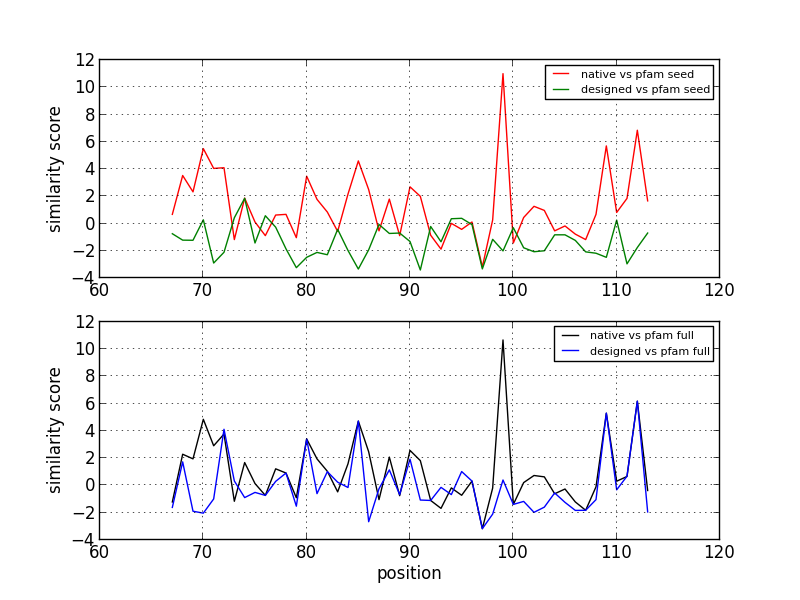
\includegraphics[width=8cm]{simil_bypos_1ABO_h.png}~
          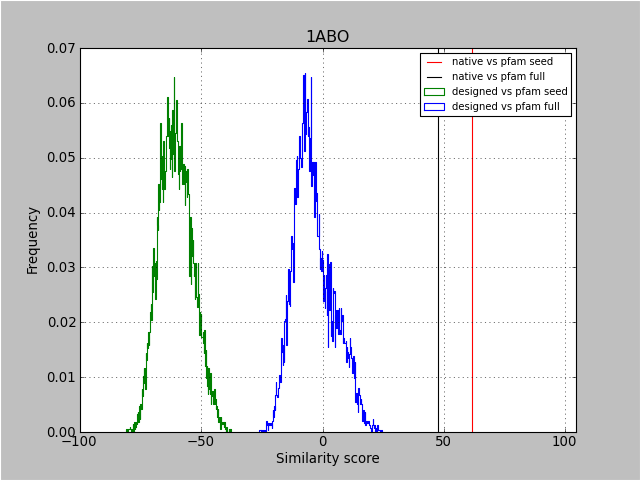
\includegraphics[width=8cm]{simil_byseq_1ABO_h.png} 
     \caption{protocole h}
   \end{subfigure}

   \begin{subfigure}[b]{\linewidth}
     \centering
          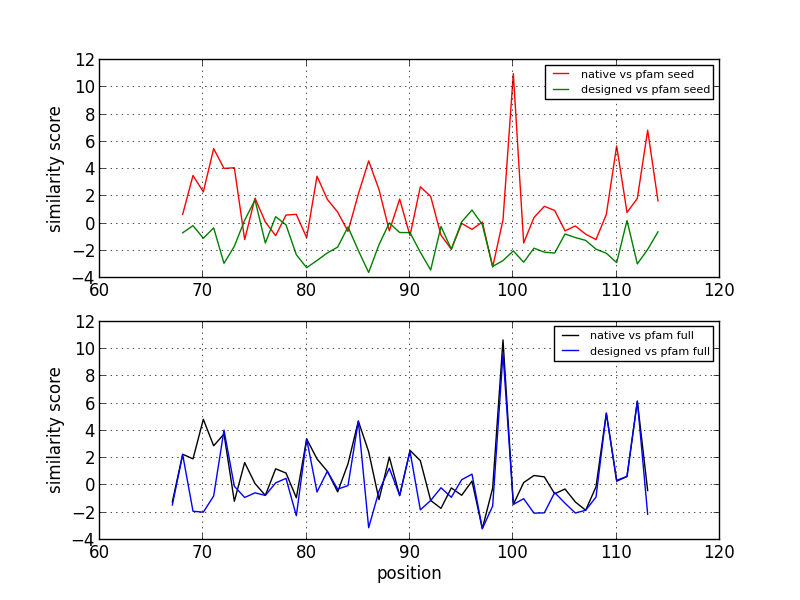
\includegraphics[width=8cm]{simil_bypos_1ABO_mc2.png}~ 
          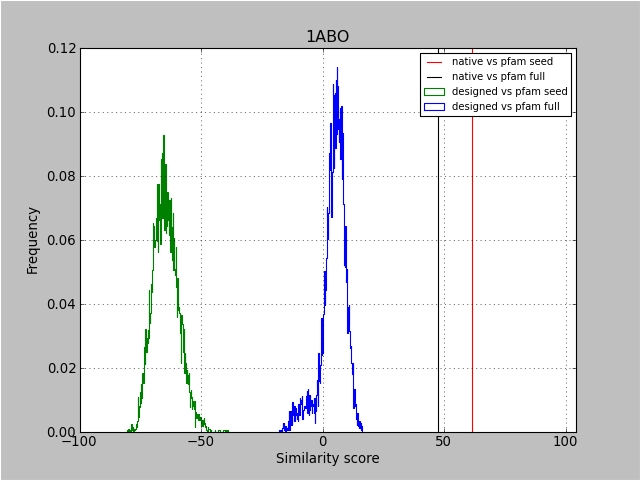
\includegraphics[width=8cm]{simil_byseq_1ABO_mc2.png} 
     \caption{protocole mc2}
   \end{subfigure}

   \begin{subfigure}[b]{\linewidth}
     \centering
          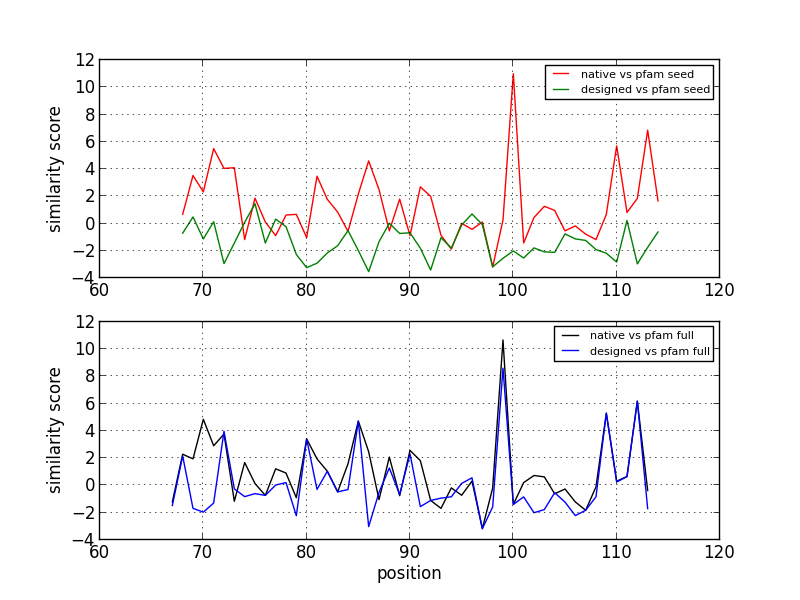
\includegraphics[width=8cm]{simil_bypos_1ABO_mc3.png}~  
          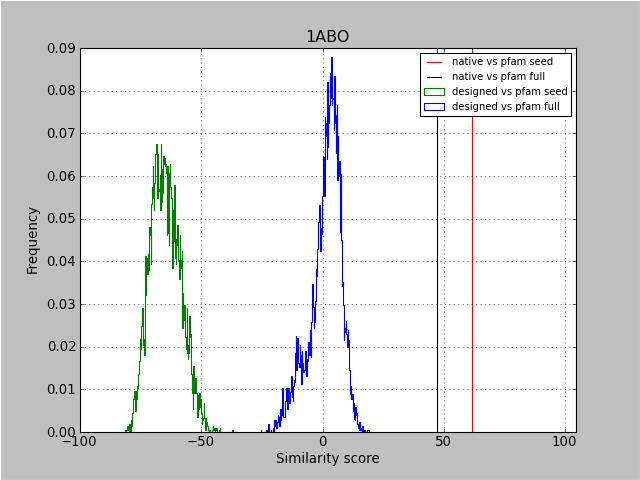
\includegraphics[width=8cm]{simil_byseq_1ABO_mc3.png} 
     \caption{protocole mc3}
   \end{subfigure}

     \caption{Similarité par position et par séquence pour 1ABO}
\label{grah:simil_1ABO}
   \end{figure}

   \begin{figure}
   \begin{subfigure}[b]{\linewidth}
     \centering
          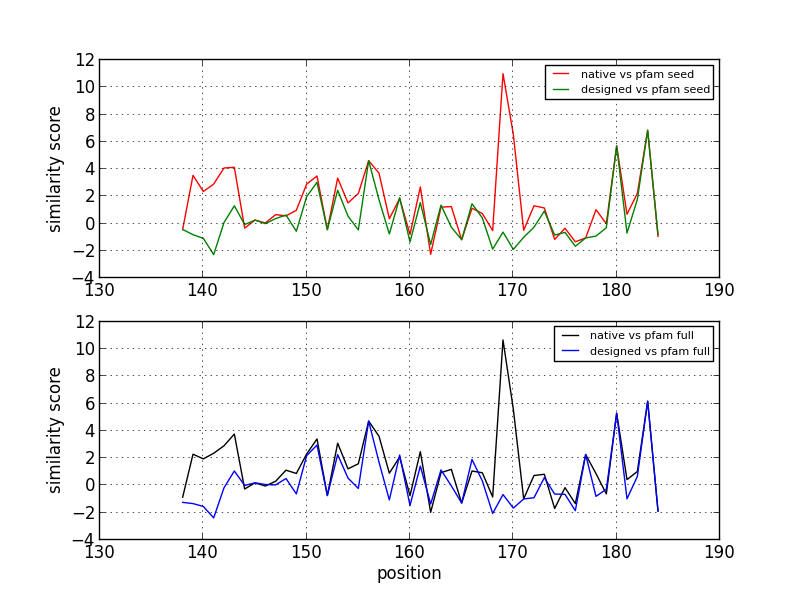
\includegraphics[width=8cm]{simil_bypos_1CKA_h.png}~
          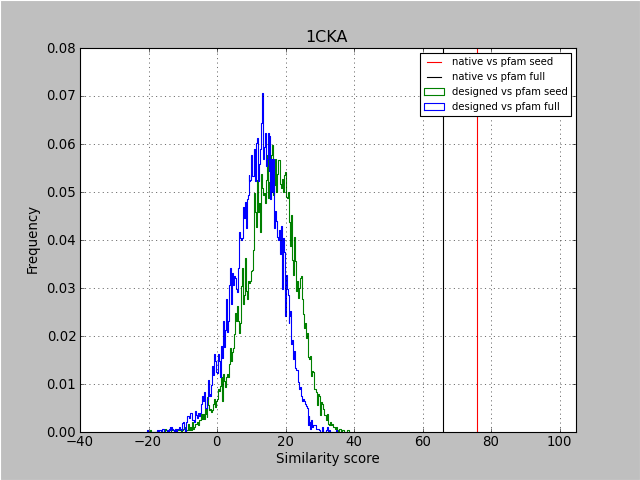
\includegraphics[width=8cm]{simil_byseq_1CKA_h.png} 
     \caption{protocole h}
   \end{subfigure}

   \begin{subfigure}[b]{\linewidth}
     \centering
          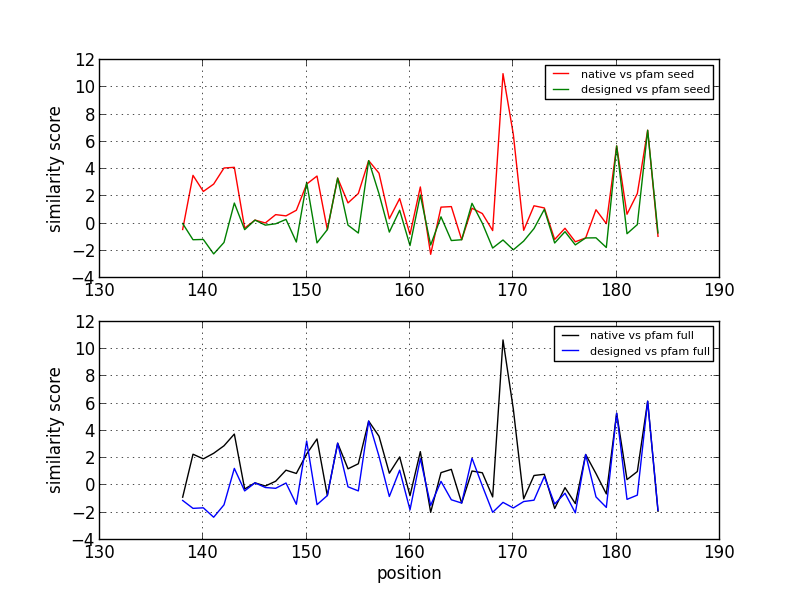
\includegraphics[width=8cm]{simil_bypos_1CKA_mc2.png}~ 
          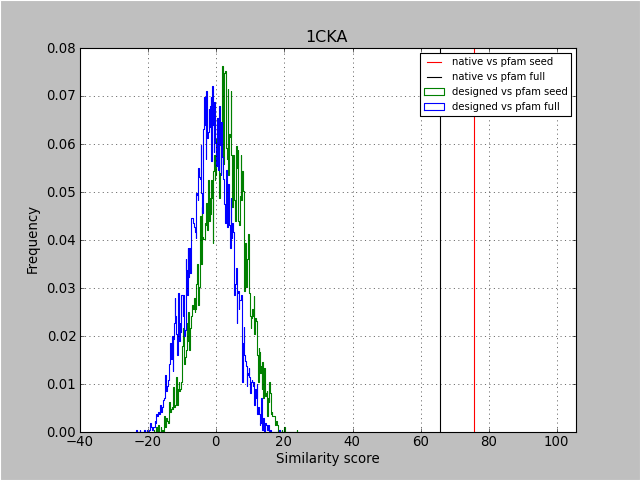
\includegraphics[width=8cm]{simil_byseq_1CKA_mc2.png} 
     \caption{protocole mc2}
   \end{subfigure}

   \begin{subfigure}[b]{\linewidth}
     \centering
          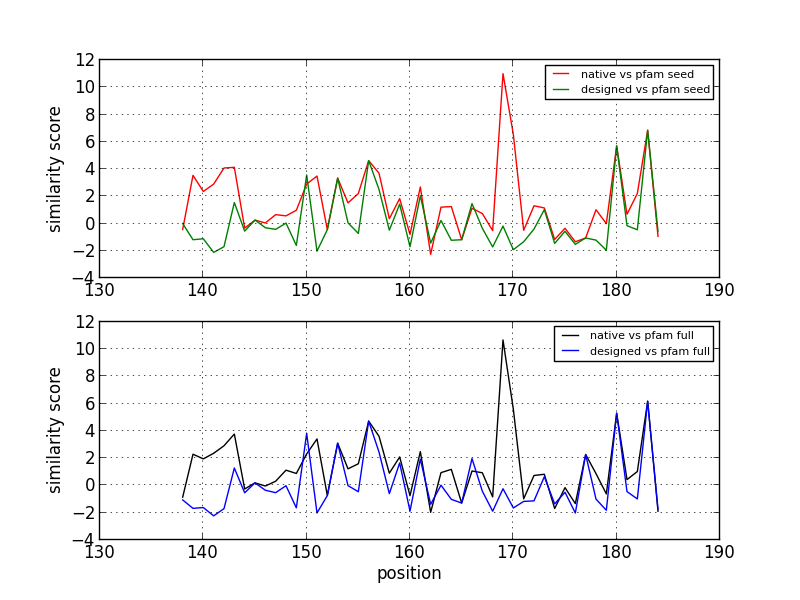
\includegraphics[width=8cm]{simil_bypos_1CKA_mc3.png}~  
          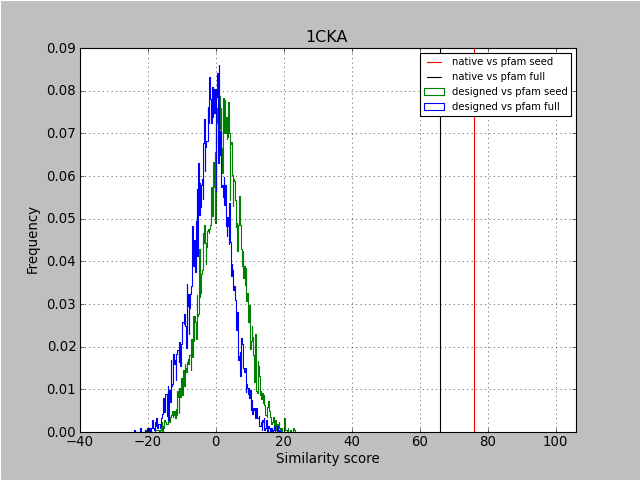
\includegraphics[width=8cm]{simil_byseq_1CKA_mc3.png} 
     \caption{protocole mc3}
   \end{subfigure}

     \caption{Similarité par position et par séquence pour 1CKA}
\label{grah:simil_1CKA}
   \end{figure}

   \begin{figure}
   \begin{subfigure}[b]{\linewidth}
     \centering
          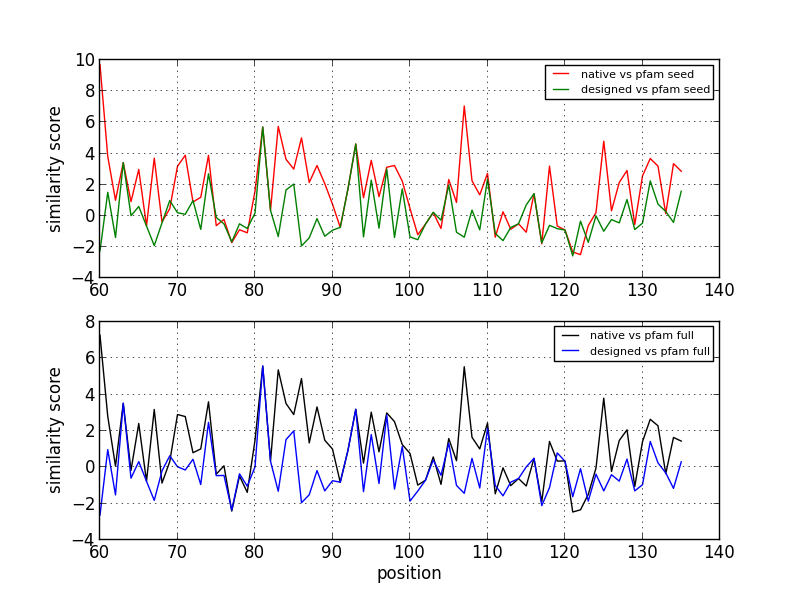
\includegraphics[width=8cm]{simil_bypos_1BM2_h.png}~
          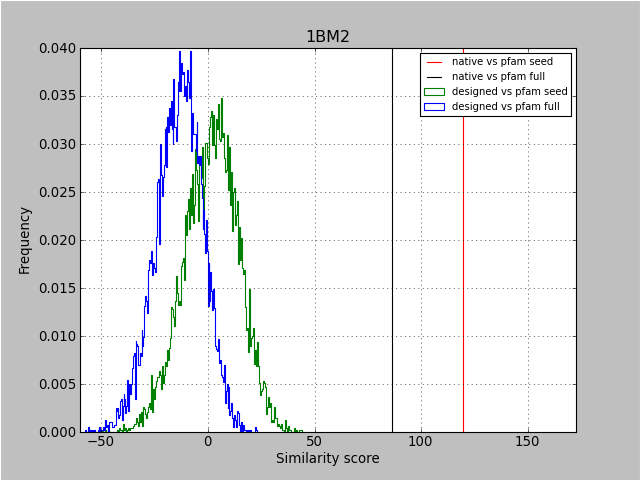
\includegraphics[width=8cm]{simil_byseq_1BM2_h.png} 
     \caption{protocole h}
   \end{subfigure}

   \begin{subfigure}[b]{\linewidth}
     \centering
          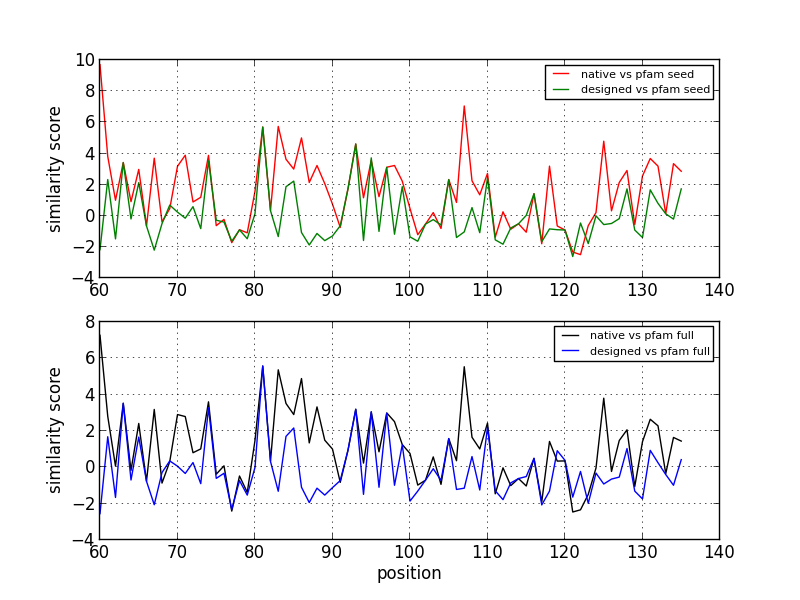
\includegraphics[width=8cm]{simil_bypos_1BM2_mc2.png}~ 
          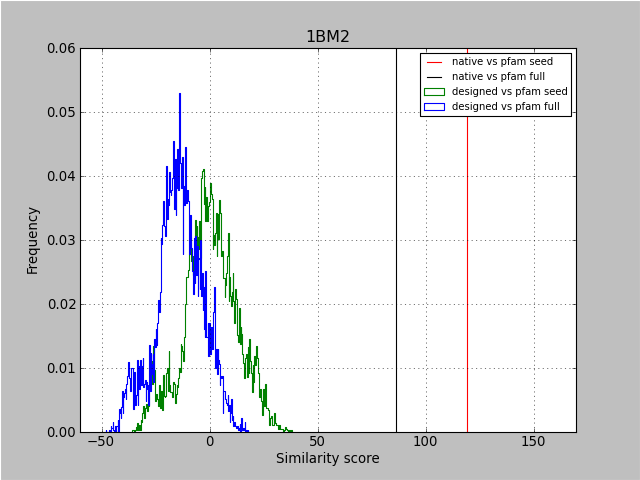
\includegraphics[width=8cm]{simil_byseq_1BM2_mc2.png} 
     \caption{protocole mc2}
   \end{subfigure}

   \begin{subfigure}[b]{\linewidth}
     \centering
          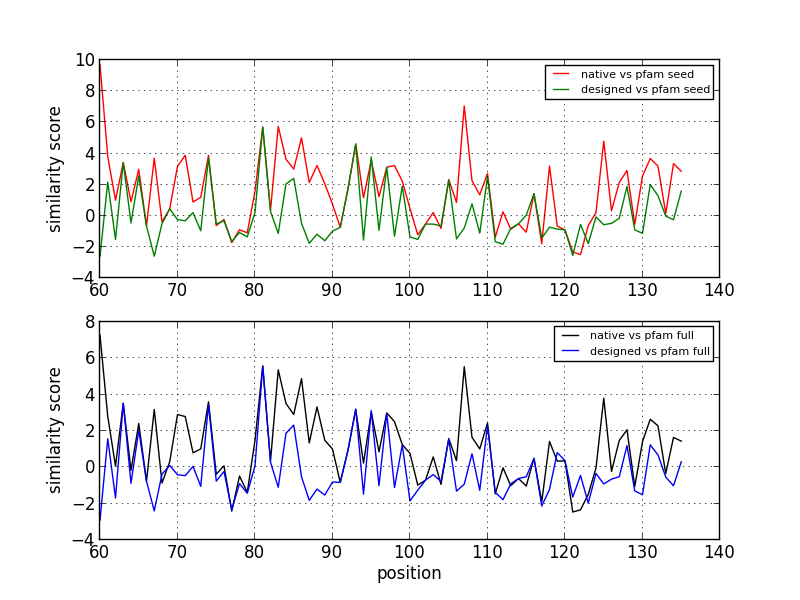
\includegraphics[width=8cm]{simil_bypos_1BM2_mc3.png}~  
          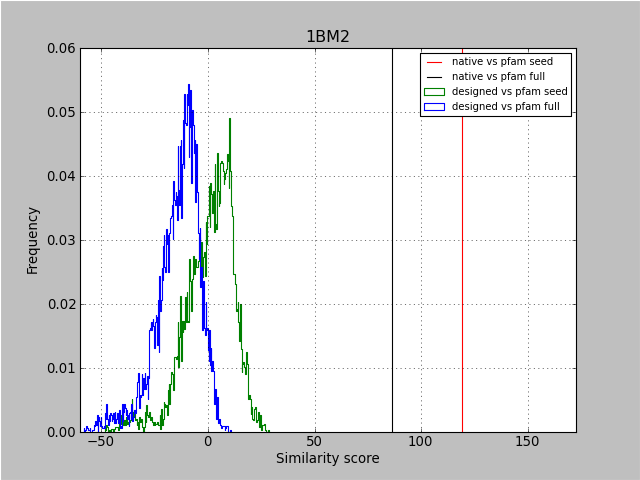
\includegraphics[width=8cm]{simil_byseq_1BM2_mc3.png} 
     \caption{protocole mc3}
   \end{subfigure}

     \caption{Similarité par position et par séquence pour 1BM2}
\label{grah:simil_1BM2}
   \end{figure}

   \begin{figure}
   \begin{subfigure}[b]{\linewidth}
     \centering
          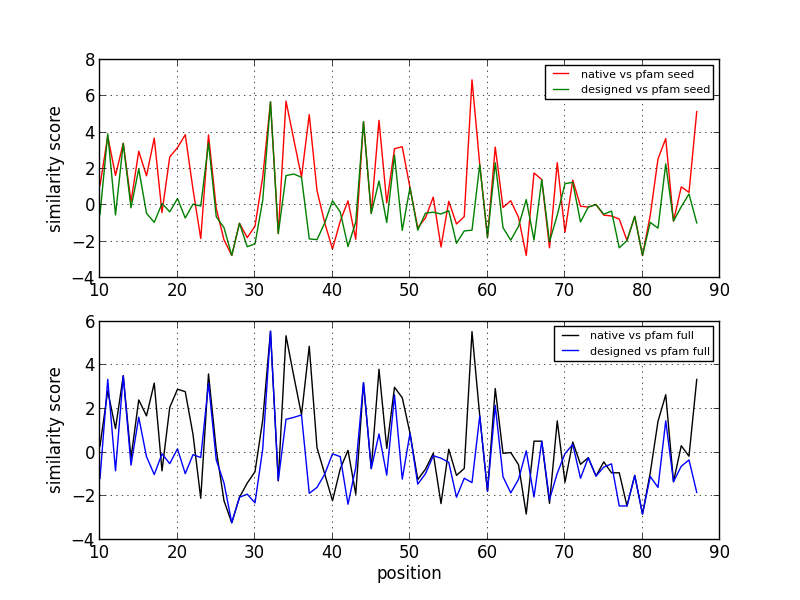
\includegraphics[width=8cm]{simil_bypos_1M61_h.png}~
          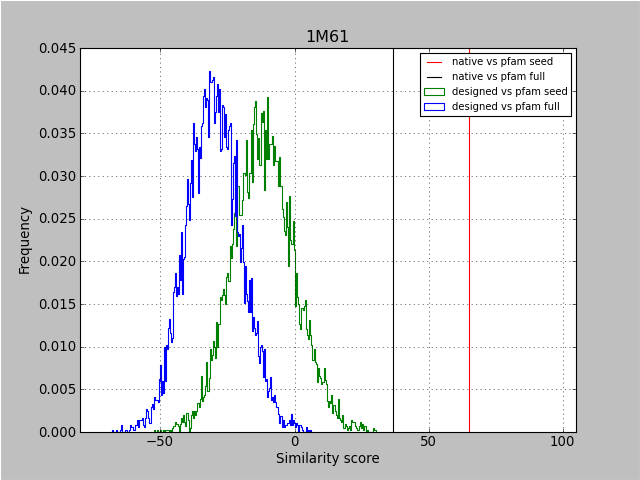
\includegraphics[width=8cm]{simil_byseq_1M61_h.png} 
     \caption{protocole h}
   \end{subfigure}

   \begin{subfigure}[b]{\linewidth}
     \centering
          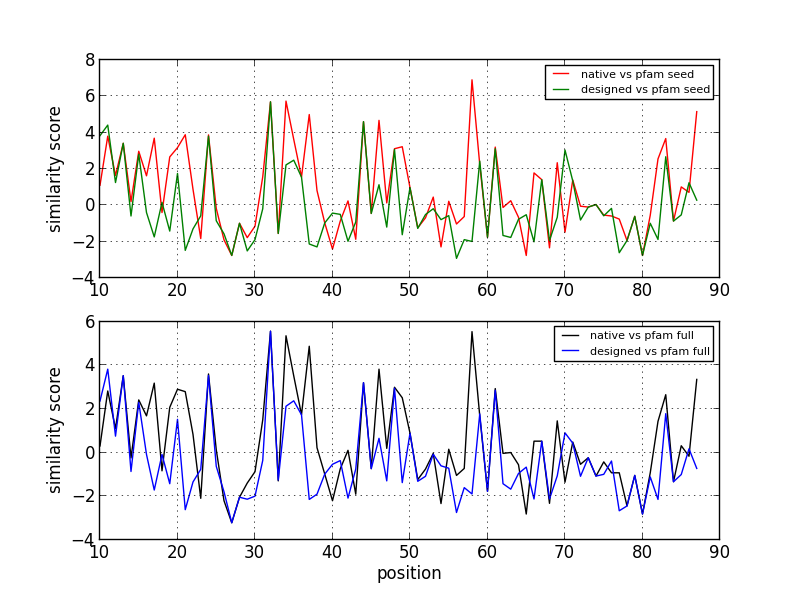
\includegraphics[width=8cm]{simil_bypos_1M61_mc2.png}~ 
          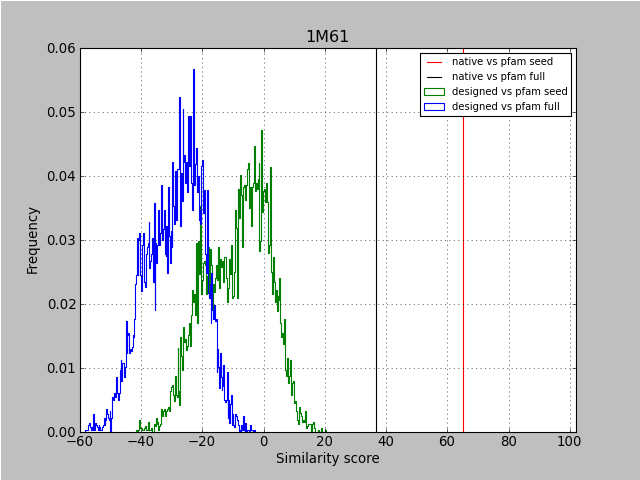
\includegraphics[width=8cm]{simil_byseq_1M61_mc2.png} 
     \caption{protocole mc2}
   \end{subfigure}

   \begin{subfigure}[b]{\linewidth}
     \centering
          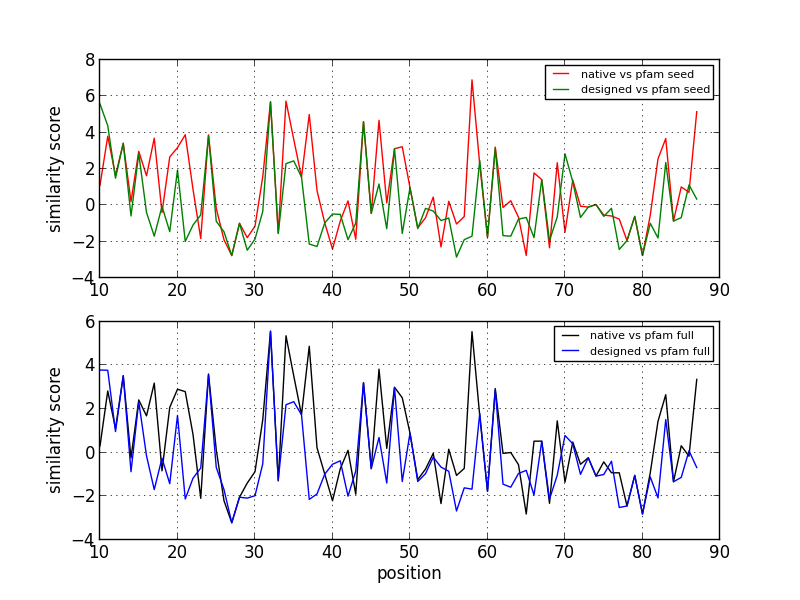
\includegraphics[width=8cm]{simil_bypos_1M61_mc3.png}~  
          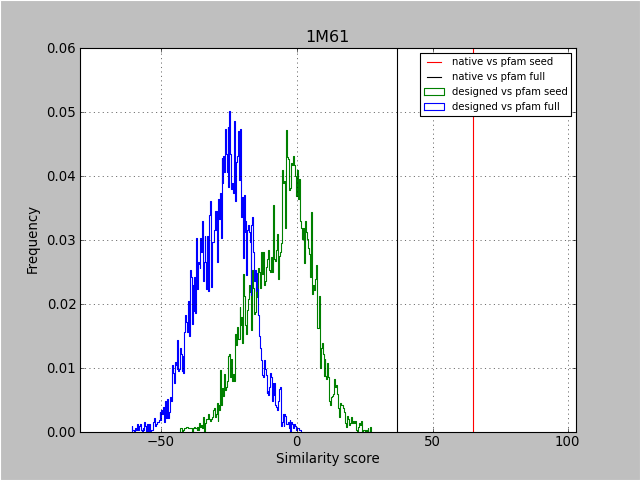
\includegraphics[width=8cm]{simil_byseq_1M61_mc3.png} 
     \caption{protocole mc3}
   \end{subfigure}

     \caption{Similarité par position et par séquence pour 1M61}
\label{grah:simil_1M61}
   \end{figure}

   \begin{figure}
   \begin{subfigure}[b]{\linewidth}
     \centering
          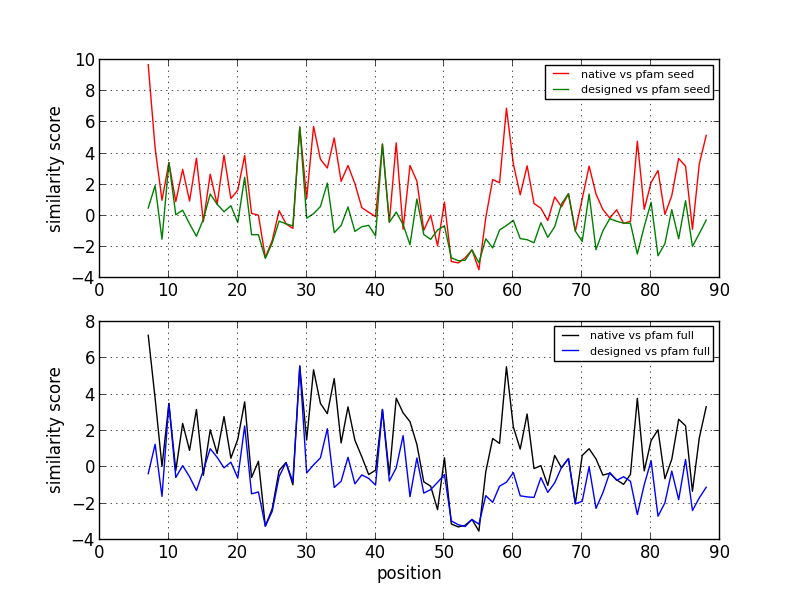
\includegraphics[width=8cm]{simil_bypos_1O4C_h.png}~
          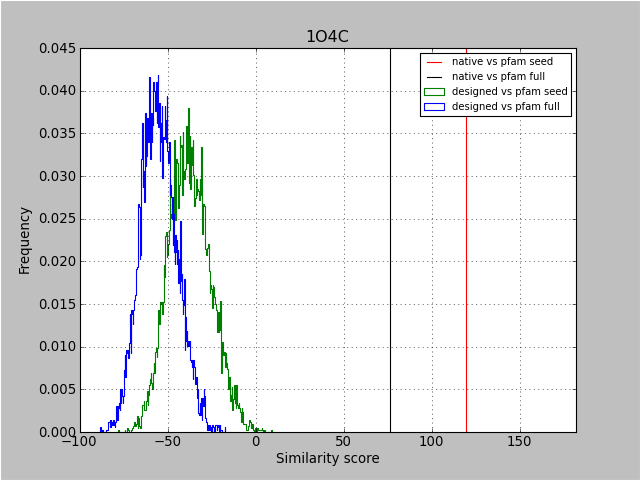
\includegraphics[width=8cm]{simil_byseq_1O4C_h.png} 
     \caption{protocole h}
   \end{subfigure}

   \begin{subfigure}[b]{\linewidth}
     \centering
          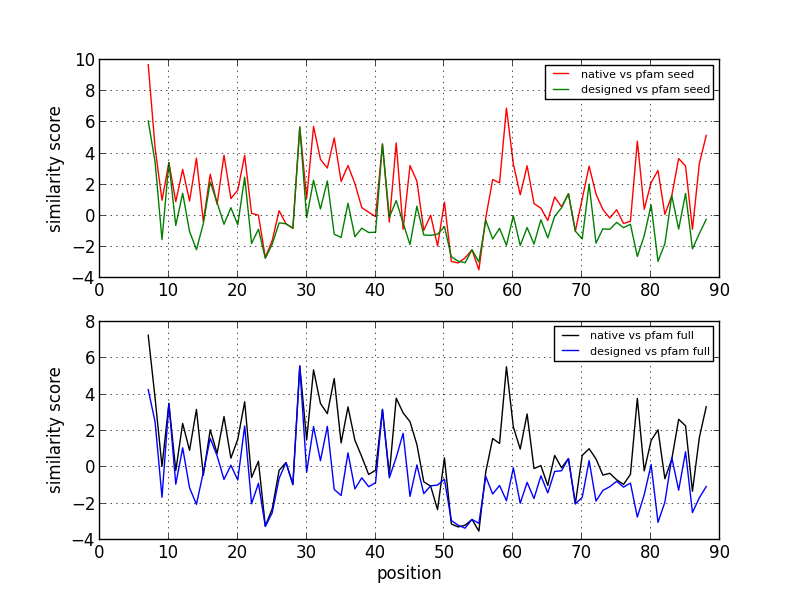
\includegraphics[width=8cm]{simil_bypos_1O4C_mc2.png}~ 
          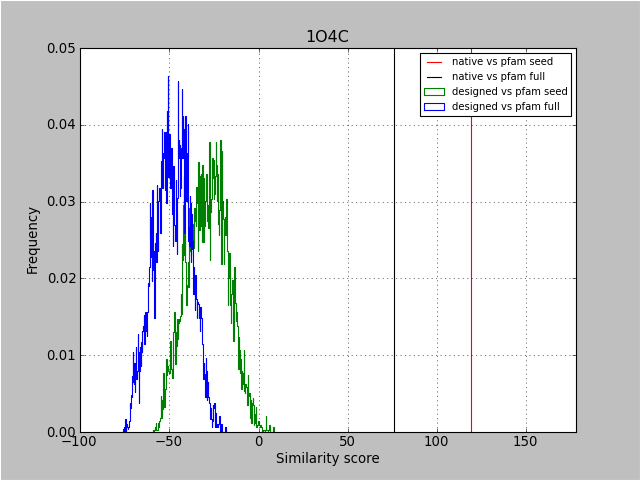
\includegraphics[width=8cm]{simil_byseq_1O4C_mc2.png} 
     \caption{protocole mc2}
   \end{subfigure}

   \begin{subfigure}[b]{\linewidth}
     \centering
          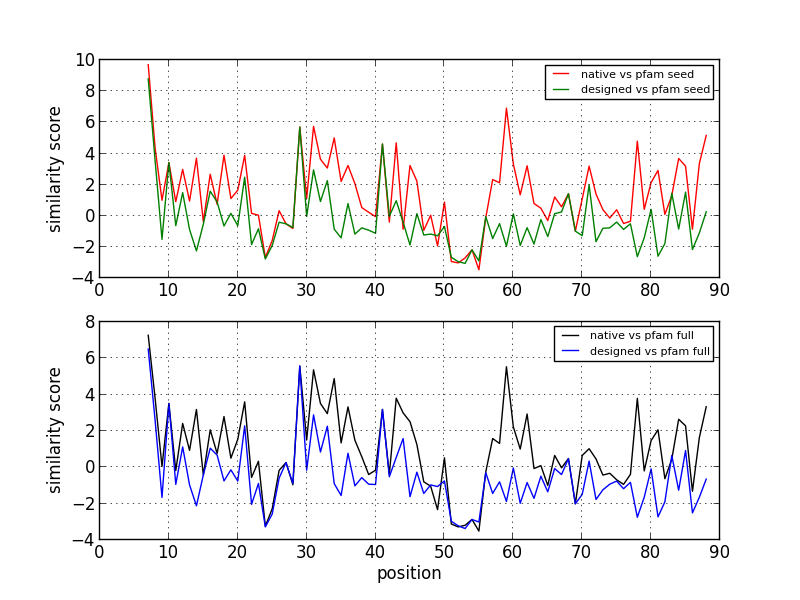
\includegraphics[width=8cm]{simil_bypos_1O4C_mc3.png}~  
          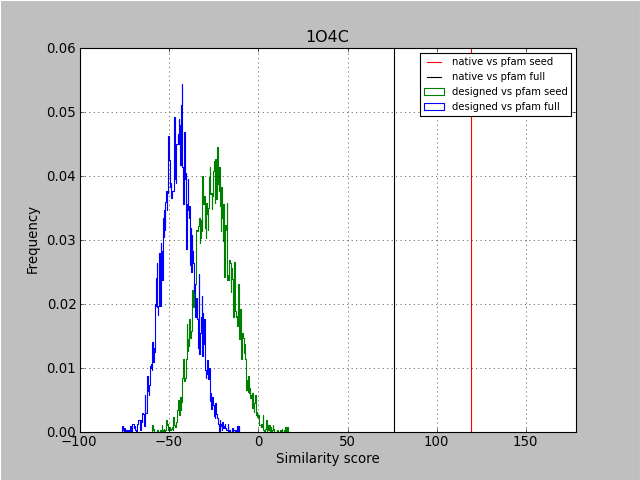
\includegraphics[width=8cm]{simil_byseq_1O4C_mc3.png} 
     \caption{protocole mc3}
   \end{subfigure}

     \caption{Similarité par position et par séquence pour 1O4C}
\label{grah:simil_1O4C}
   \end{figure}

   \begin{figure}
   \begin{subfigure}[b]{\linewidth}
     \centering
          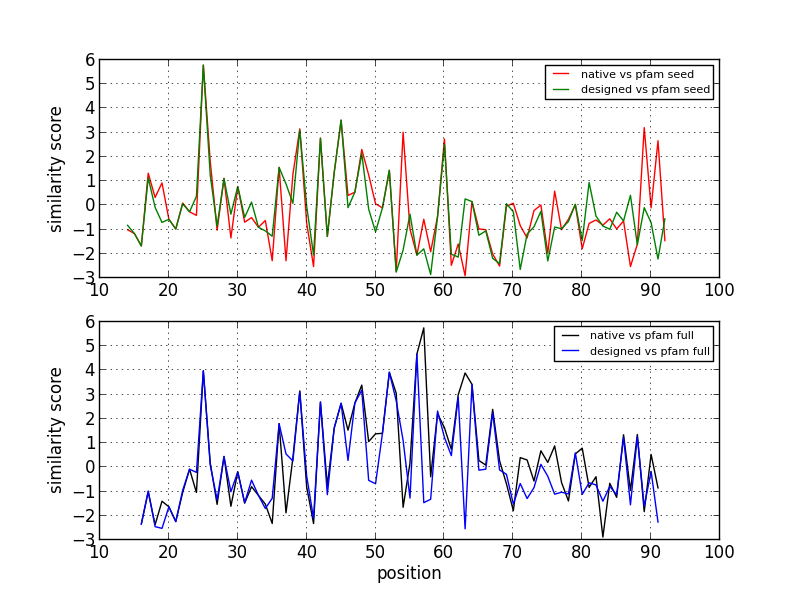
\includegraphics[width=8cm]{simil_bypos_1G9O_h.png}~
          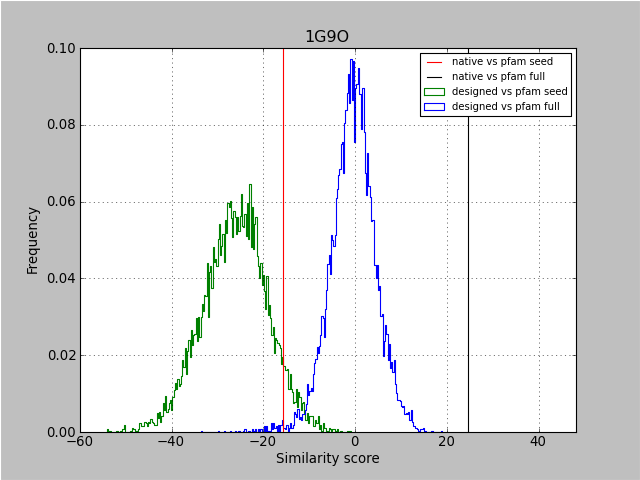
\includegraphics[width=8cm]{simil_byseq_1G9O_h.png} 
     \caption{protocole h}
   \end{subfigure}

   \begin{subfigure}[b]{\linewidth}
     \centering
          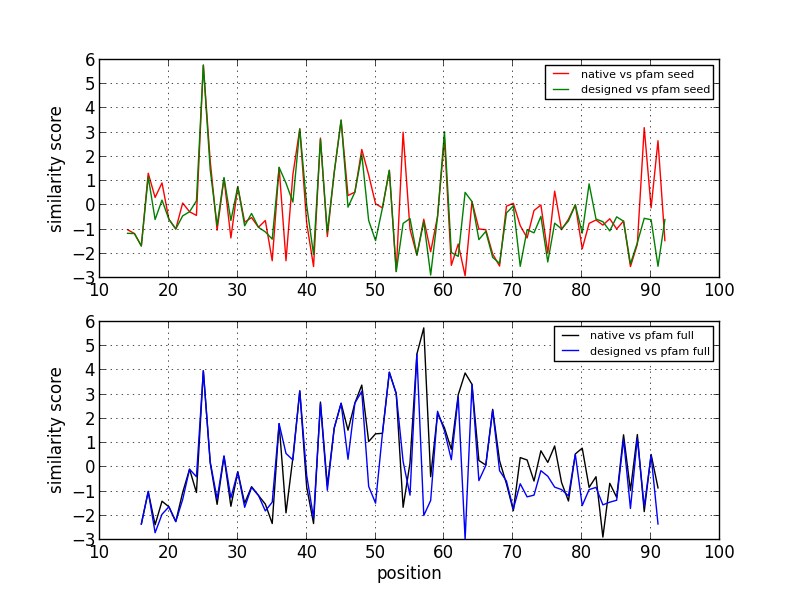
\includegraphics[width=8cm]{simil_bypos_1G9O_mc2.png}~ 
          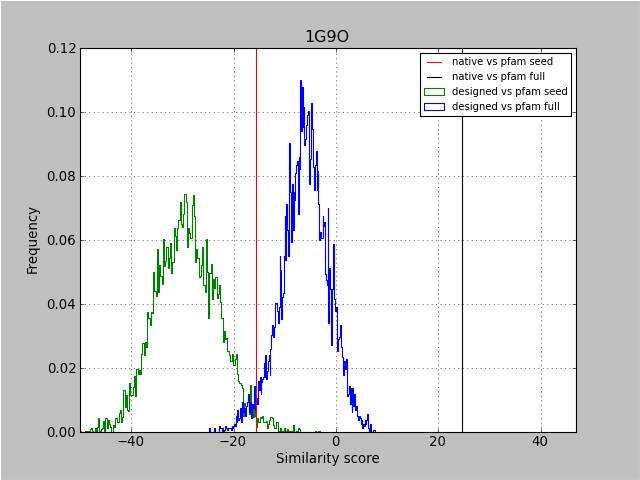
\includegraphics[width=8cm]{simil_byseq_1G9O_mc2.png} 
     \caption{protocole mc2}
   \end{subfigure}

   \begin{subfigure}[b]{\linewidth}
     \centering
          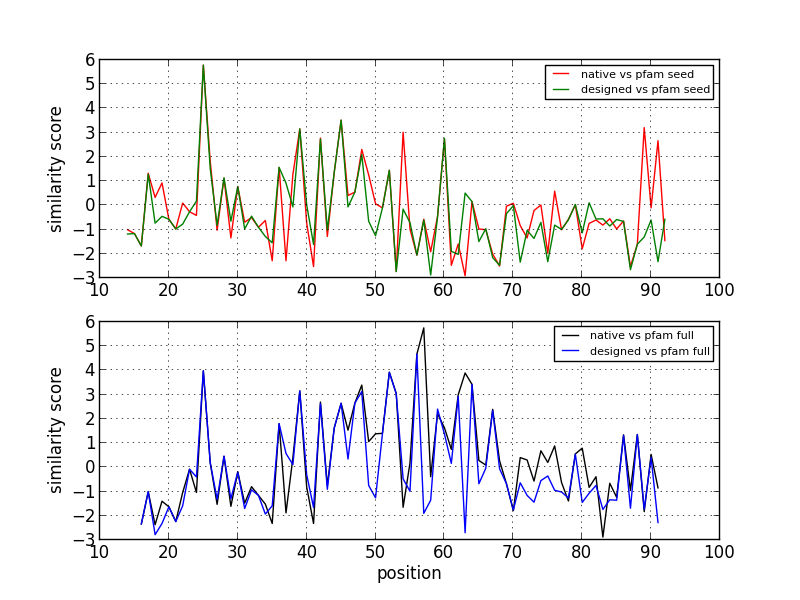
\includegraphics[width=8cm]{simil_bypos_1G9O_mc3.png}~  
          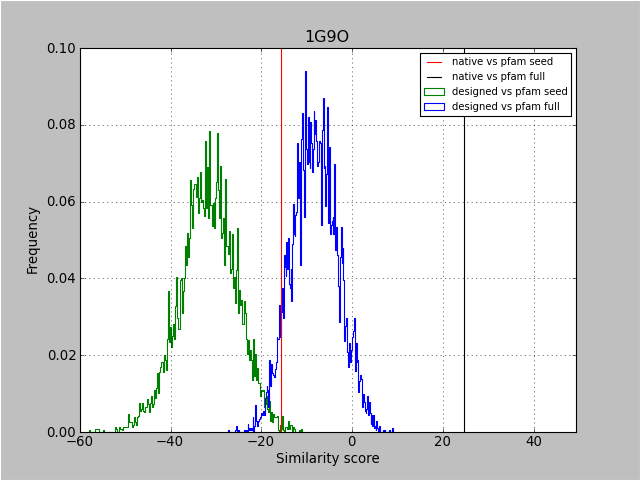
\includegraphics[width=8cm]{simil_byseq_1G9O_mc3.png} 
     \caption{protocole mc3}
   \end{subfigure}

     \caption{Similarité par position et par séquence pour 1G9O}
\label{grah:simil_1G9O}
   \end{figure}

   \begin{figure}
   \begin{subfigure}[b]{\linewidth}
     \centering
          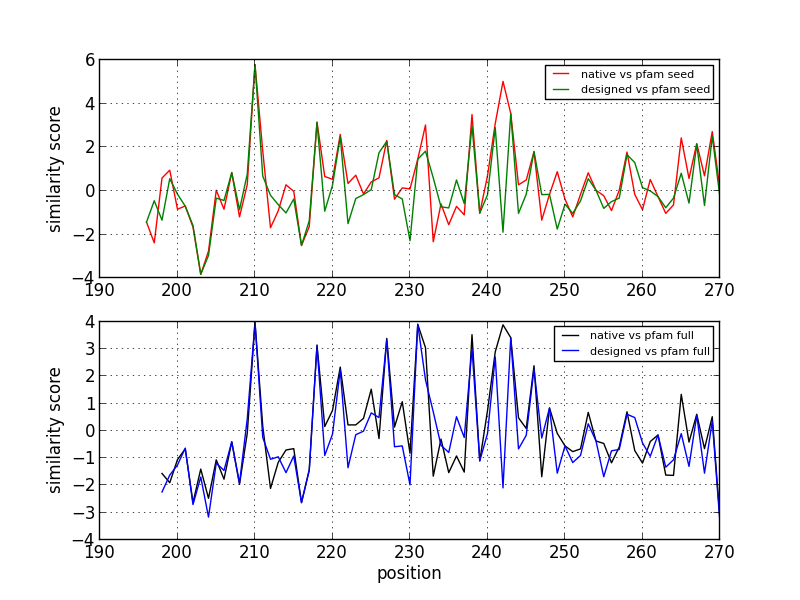
\includegraphics[width=8cm]{simil_bypos_1R6J_h.png}~
          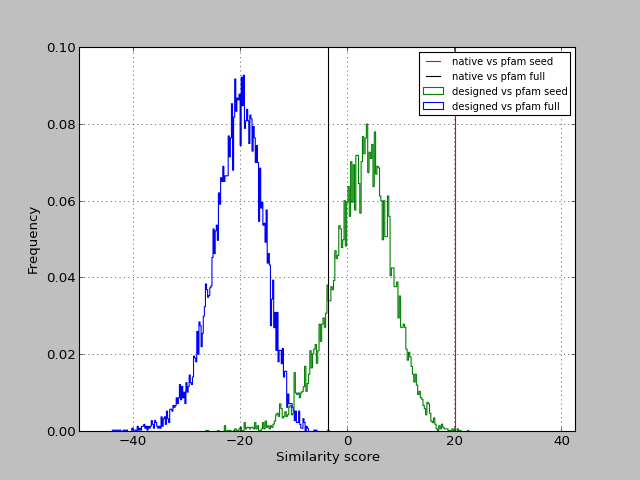
\includegraphics[width=8cm]{simil_byseq_1R6J_h.png} 
     \caption{protocole h}
   \end{subfigure}

   \begin{subfigure}[b]{\linewidth}
     \centering
          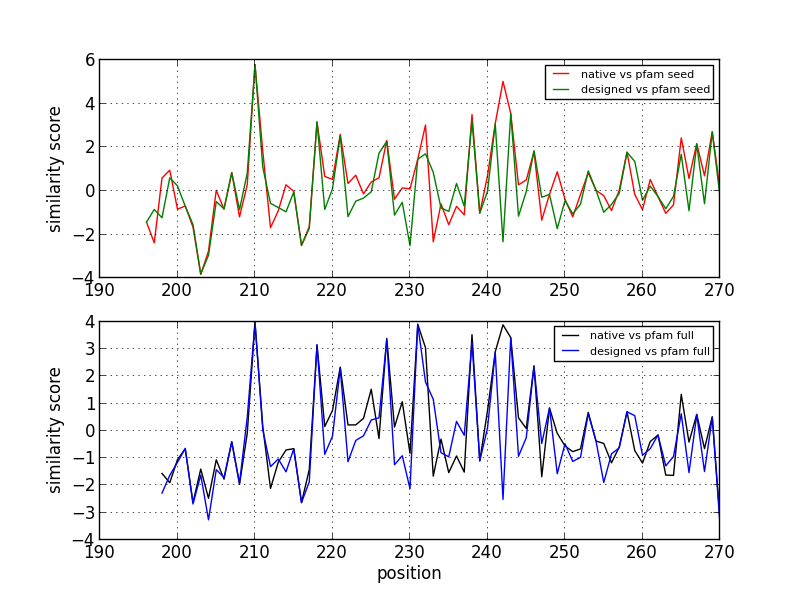
\includegraphics[width=8cm]{simil_bypos_1R6J_mc2.png}~ 
          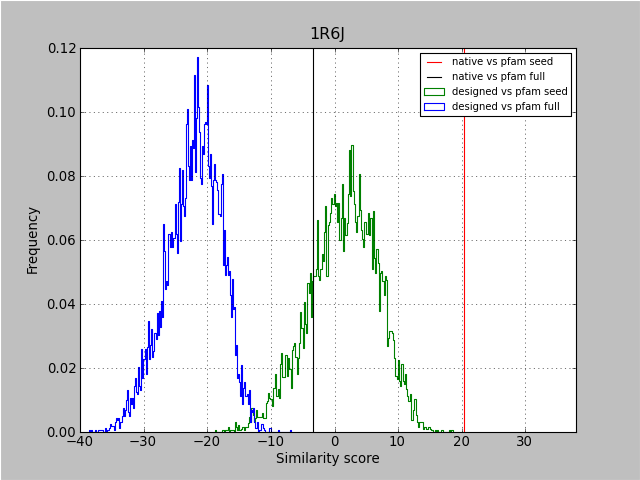
\includegraphics[width=8cm]{simil_byseq_1R6J_mc2.png} 
     \caption{protocole mc2}
   \end{subfigure}

   \begin{subfigure}[b]{\linewidth}
     \centering
          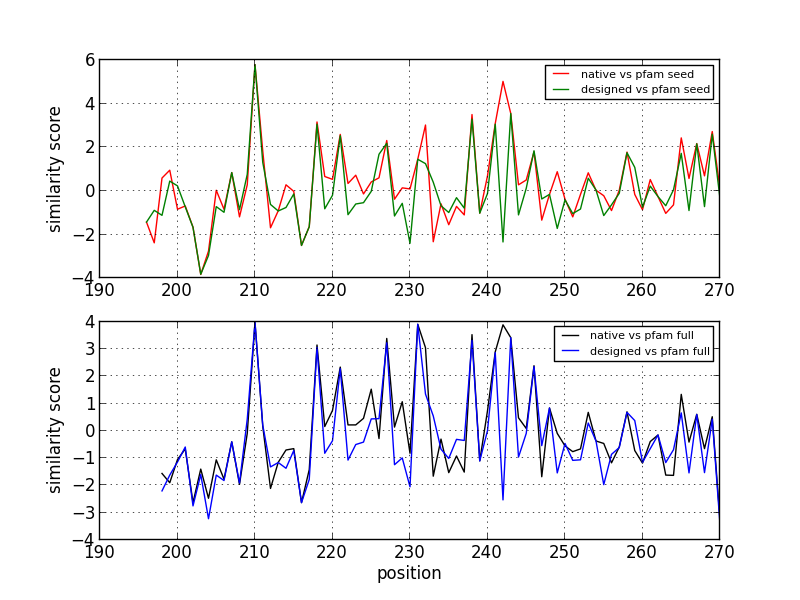
\includegraphics[width=8cm]{simil_bypos_1R6J_mc3.png}~  
          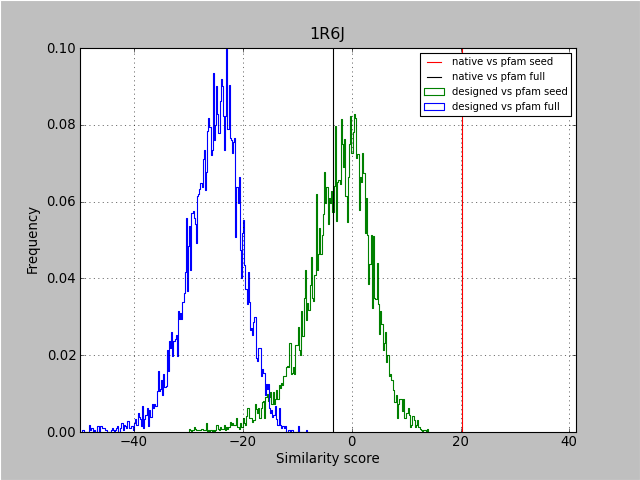
\includegraphics[width=8cm]{simil_byseq_1R6J_mc3.png} 
     \caption{protocole mc3}
   \end{subfigure}

     \caption{Similarité par position et par séquence pour 1R6J}
\label{grah:simil_1R6J}
   \end{figure}

         \subsubsection{rapport entre énergies et  similarités}
Pour faire le lien entre les comparaisons basées sur les meilleurs énergies et les comparaisons basées sur les scores de similarités, nous représentons les énergies des dix milles meilleurs séquences en fonction de leur similarité à l'alignement Pfam \og seed\fg. Comme une séquence peut apparaître plusieurs fois dans l'ensemble des séquences/conformations obtenus toutes les énergies trouvées de la séquence sont représentées voir les graphiques \ref{graph:simil_vs_ener}. La corrélation entre les deux critères semble très faible.Pour 1CKA malgré des énergies pour l'heuristique moins bonnes, la similarité est meilleur.Bien que les énergies obtenues avec le protocole mc2 soient meilleurs que celles avec le protocole mc3, il n'y a pas de différences significatives sur les scores de similarités obtenus.

   \begin{figure}[t]
     \centering
     \begin{tabular}{cc}
       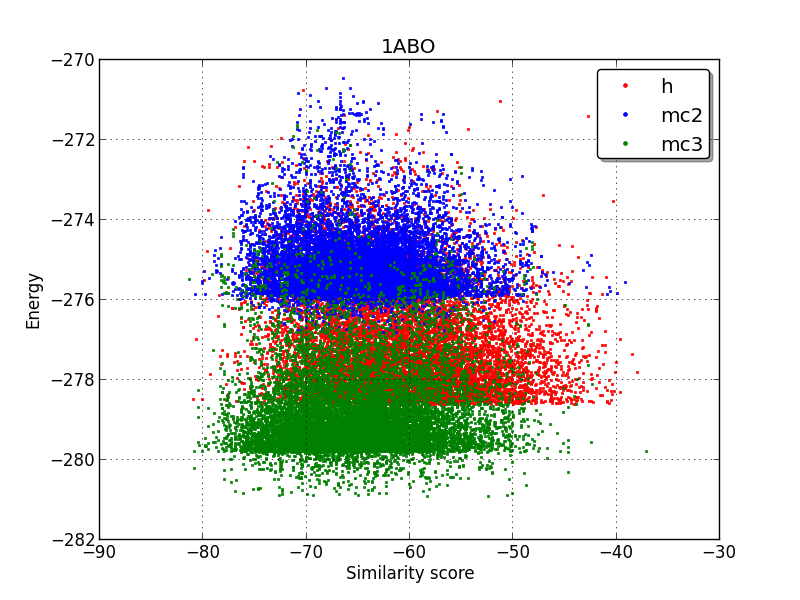
\includegraphics[width=7cm]{simil_vs_ener_1ABO.png} &
       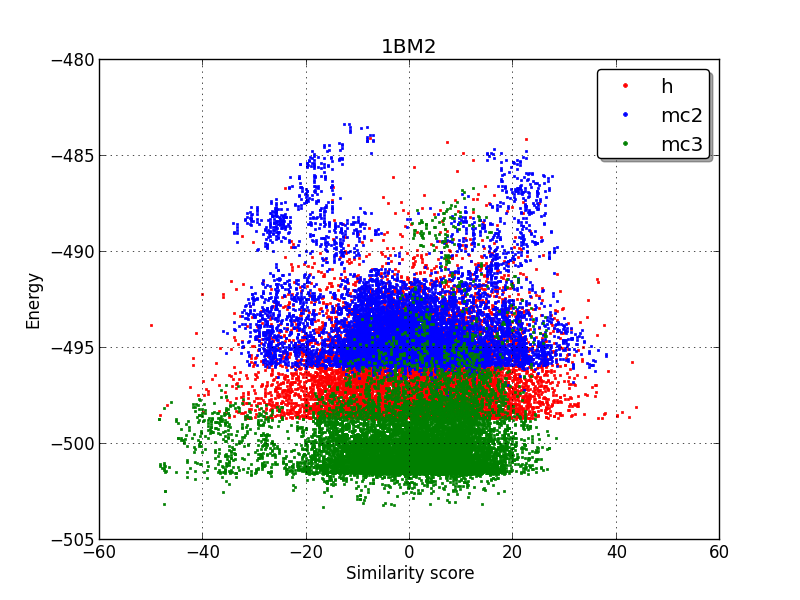
\includegraphics[width=7cm]{simil_vs_ener_1BM2.png} \\
       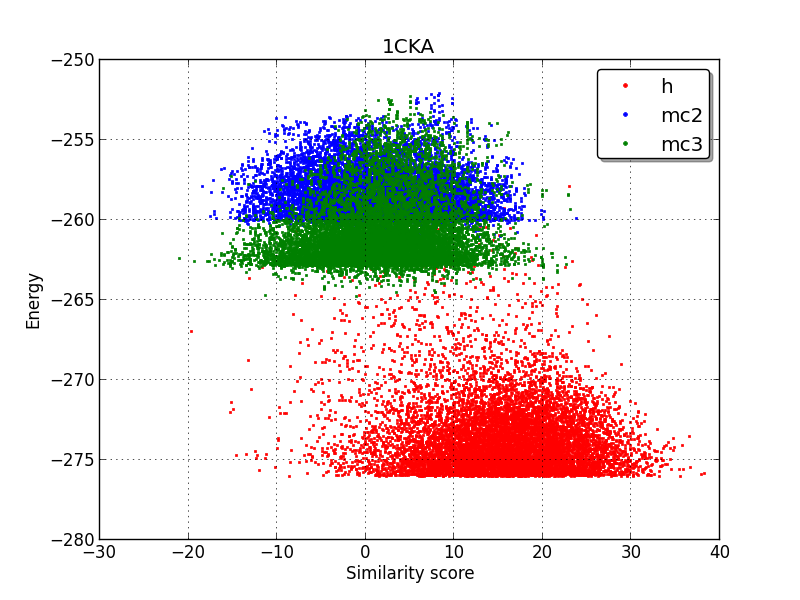
\includegraphics[width=7cm]{simil_vs_ener_1CKA.png} &
       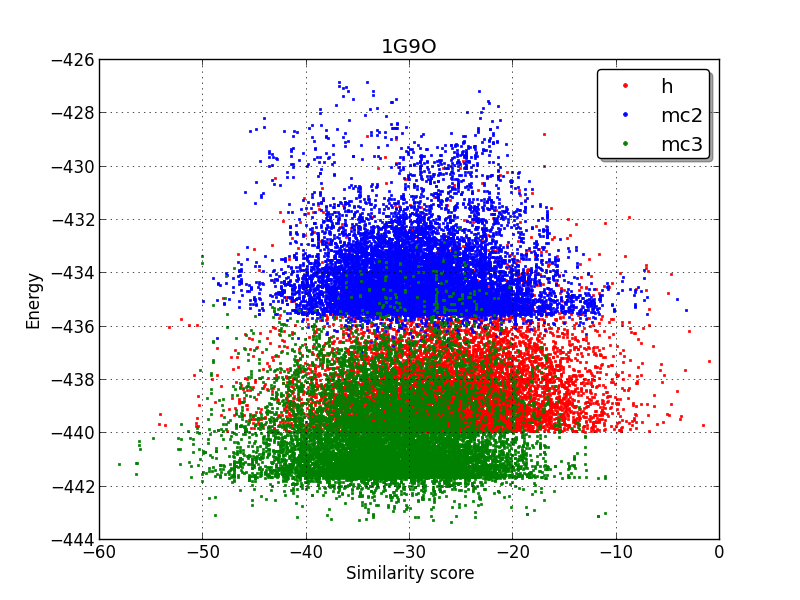
\includegraphics[width=7cm]{simil_vs_ener_1G9O.png} \\
       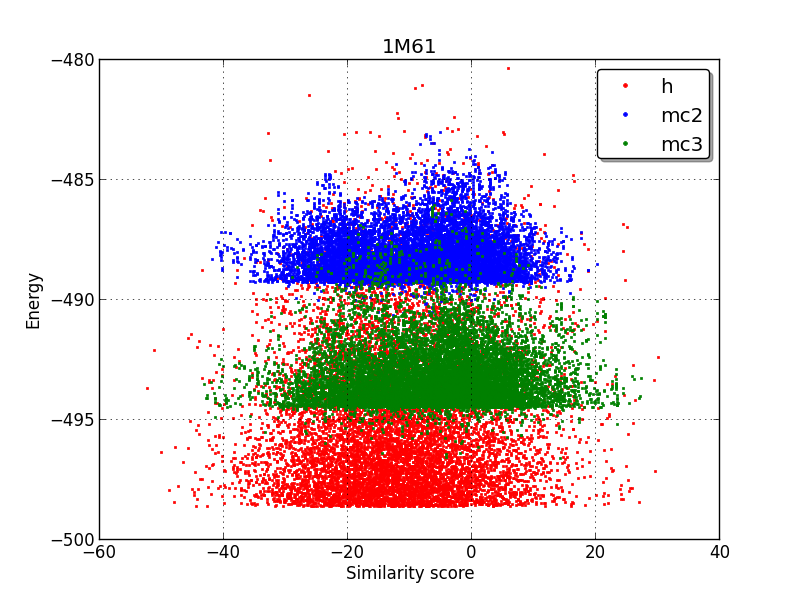
\includegraphics[width=7cm]{simil_vs_ener_1M61.png} &
       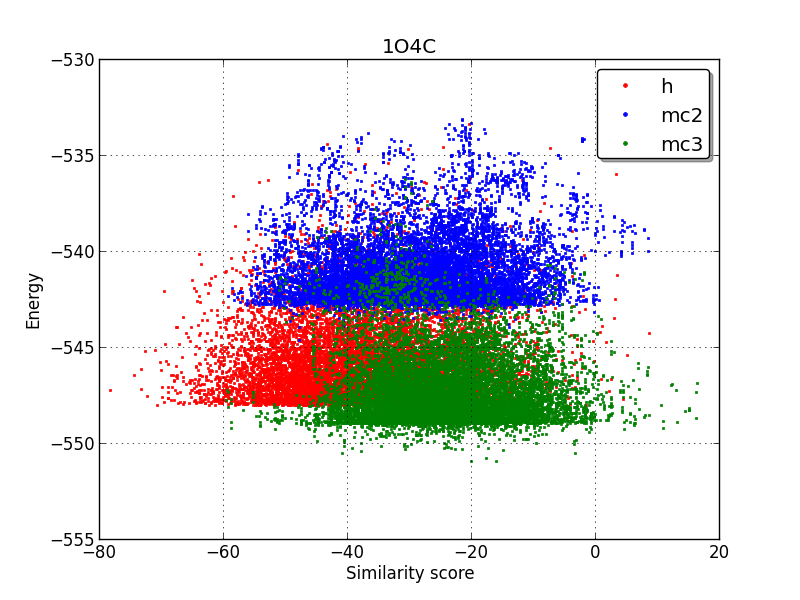
\includegraphics[width=7cm]{simil_vs_ener_1O4C.png} \\
       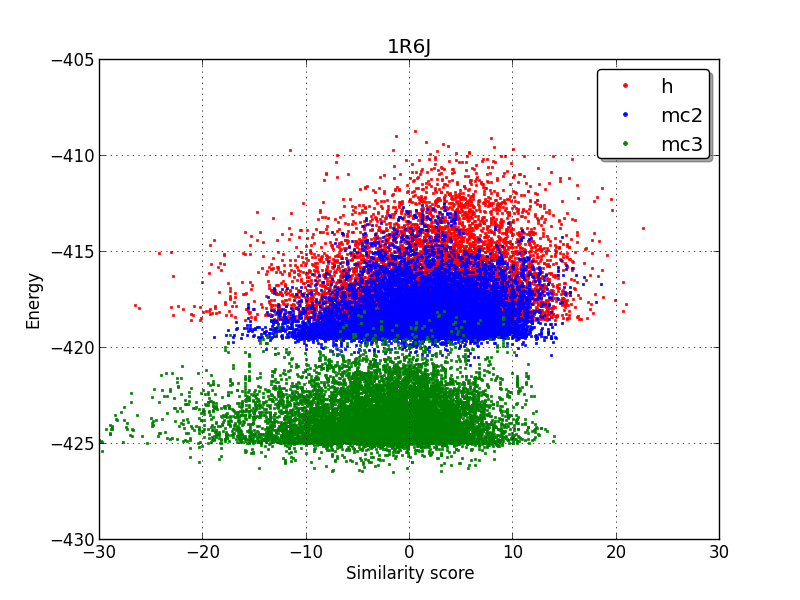
\includegraphics[width=8cm]{simil_vs_ener_1R6J.png} \\
     \end{tabular}
     
     \caption{}
\label{graph:simil_vs_ener}
   \end{figure}
 

         \subsubsection{Comparaisons des distributions selon l'énergie}

Ici nous nous intéressons aux ensembles de cent mille séquences/conformations de meilleurs énergies.Nous calculons les centiles d'énergie pour chaque protéine et pour chacun des trois protocoles h , mc2, mc3.  

Les figures~\ref{graph:centiles} représentent la répartition des énergies selon les centiles, ceci pour les trois protocoles h, mc2, mc3. Pour le premier centile  ( c'est-à-dire l'énergie au dessus de la quelle il y a les milles meilleurs séquences/conformations) le protocole mc2 domine sauf pour la protéine 1R6J où h est meilleur jusqu'au vingtième centile .Pour 1ABO, alors que mc2 et mc3 font quasiment jeu égal pour la meilleur énergie, le premier centile de mc2 est nettement plus haut que celui de mc3.Mais en général, L'allure des courtes des deux protolcoles Monte-carlo est très proche et les écarts entre  les meilleurs énergies de mc2 et mc3 sont globalement conservés le long des centiles.Ce n'est pas le cas entre h et les protocoles Monte-Carlo, où l'on voit un déclin plus rapide le long des centiles.Ce qui montre une densité plus faible des séquences/conformations de bonne énergie pour l'heuristique. 



 



   \begin{figure}[t]
     \centering
     \begin{tabular}{cc}
       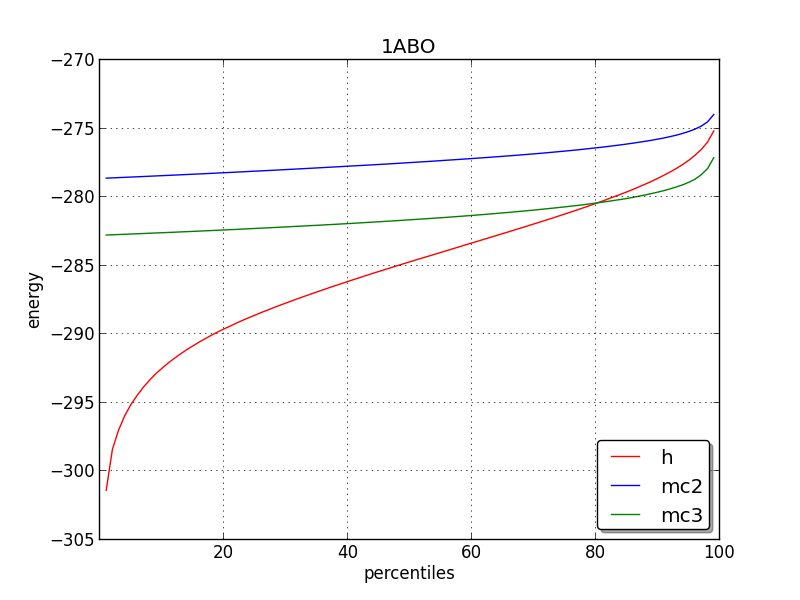
\includegraphics[width=8cm]{centiles_1ABO.png} &
       \includegraphics[width=8cm]{centiles_1BM2.png} \\
       \includegraphics[width=8cm]{centiles_1CKA.png} &
       \includegraphics[width=8cm]{centiles_1G9O.png} \\
       \includegraphics[width=8cm]{centiles_1M61.png} &
       \includegraphics[width=8cm]{centiles_1O4C.png} \\
       \includegraphics[width=8cm]{centiles_1R6J.png} \\
     \end{tabular}
     
     \caption{Distribution des 100000 meilleurs séquences selon l'énergie.}
\label{grah:centiles}
   \end{figure}
 
\clearpage

        \subsection{Comparaison avec toutes les positions actives}

Passons maintenant, aux résultats obtenus avec la seconde version de proteus~\ref{qqchose}.Cette version intègre notamment l'algorithme \og Replica Exchange\fg. Nous pouvons donc faire des comparaisons entre les trois algorithmes du programme.Tous les protocoles utilisés sont décrits dans les tableaux~\ref{tab:protoMC} ou \ref{tab:protoRE}.Commençons par la recherche de la séquence/conformation de meilleur énergie pour toutes les positions actives. Les tests sont décrits au paragraphe~\ref{methode_TTactif}. Les résultats sont présentés sous forme de tableau en~\ref{tab:best_ener_all_all} qui contient la meilleur énergie arrondie à la kcal/mol inférieure et aussi sous forme de graphique en~\ref{graph:best_ener_all_all} où sont représenter les différences par rapport à la meilleur énergie pour tous les cas. 
\subparagraph
Il n'y pas de protocoles qui domine les autres sur toutes les protéines. Le meilleur résultat est obtenu avec le protocole huit marcheurs RE8b2 pour 2BYG , 1BM2, 1O4C et 1A81, le protocole RE8b1 pour 1CKA et 1ABO, le protocole quatre marcheurs RE4b pour 1G9O , les protocoles mono-marcheur MCb pour 1M61 et H pour 1R6J.  Ces résultats sont également représentent sous forme de trois graphiques qui regroupent les protocoles utilisant les protocoles non parallèles, les protocoles quatre marcheurs et les protocoles huit marcheurs. Un quatrième graphique regroupe le meilleur protocoles de chaque algorithme. Là encore seul les différences par rapport au meilleur protocole sont représentées. Le protocole H fait jeu égale avec le meilleur protocole Monte-Carlo. Le second Monte-Carlo , qui utilise en mode de mutation moins agressif~\ref{sec:MC}, est nettement plus mauvais avec presque toujours des écarts de plus de cinq Kcal/mol avec les deux autres protocoles non parallèle.Pour le groupe de protocoles avec quatre marcheurs le RE4b ,qui se différencie des deux autres par une plage de températures la plus resserrée ,est meilleur pour cinq des sept protéines mais pour les deux protéines restantes la différences se limite à deux Kcal/mol.RE4a, le protocole avec la plage de température la large est moins bon que les autres. En ce qui conserve les protocoles huit marcheurs , deux d'entre-eux se démarquent RE8b1 et RE8b2 (plage de température resserré,grande période de swap et mode de mutation agressif pour le premier , plus conservateur pour le second). RE8b1 obtient des résultats assez irrégulier selon les protéines du meilleur pour 1CKA et 1ABO jusqu'à s'écarter de près de huit Kcal/mol de la plus haute énergie.RE8b2, soit donne les meilleurs résultats (dans cinquante pourcent des cas), soit s'écarte d'au plus quatre Kcal/mol des meilleurs résultats.  

    \begin{table}[h]
      \centering

      \begin{tabular}{cccccccccccc}


        \toprule
        Protéine & H & MCa & MCb & RE4a & RE4b & RE4c & RE8a1 & RE8a2 & RE8b1 & RE8b2 & RE8b3 \\
        \cmidrule{1-12}
        1A81 & -521 & -538 & -522 & -525 & -520 & -518 & -520 & -520 & -514 & -512 & -512 \\
        1ABO & -272 & -274 & -268 & -273 & -269 & -272 & -273 & -273 & -268 & -271 & -271 \\
        1BM2 & -484 & -500 & -486 & -488 & -481 & -486 & -489 & -489 & -478 & -476 & -480 \\
        1CKA & -252 & -258 & -249 & -259 & -251 & -249 & -251 & -251 & -247 & -248 & -252 \\
        1G9O & -428 & -435 & -428 & -429 & -421 & -428 & -430 & -430 & -428 & -425 & -426 \\
        1M61 & -480 & -493 & -479 & -483 & -480 & -480 & -481 & -481 & -480 & -480 & -480 \\
        1O4C & -535 & -545 & -531 & -536 & -529 & -532 & -536 & -536 & -527 & -524 & -525 \\
        1R6J & -407 & -419 & -414 & -415 & -409 & -414 & -411 & -411 & -409 & -408 & -409 \\
        2BYG & -457 & -469 & -454 & -461 & -456 & -462 & -460 & -460 & -456 & -454 & -454 \\
        
        \bottomrule


      \end{tabular}      
      \caption{les meilleures énergies pour tous les résidus actifs}
\label{tab:best_ener_all_all}      
    \end{table}


   \begin{figure}[t]
     \centering
     \begin{tabular}{cc}
       \includegraphics[width=18cm]{best_all.png} \\
     \end{tabular}
     \caption{Les différences entre les meilleurs énergie de chaque protocoles.}
\label{graph:best_ener_all_all}
   \end{figure}


    \clearpage


   \begin{figure}[t]
     \centering
     \begin{tabular}{cc}
       \includegraphics[width=8cm]{best_by_cat.png} &
       \includegraphics[width=8cm]{monoM.png} \\
       \includegraphics[width=8cm]{best_RE4.png} &
       \includegraphics[width=8cm]{best_RE8.png} \\
     \end{tabular}
     \caption{.Les différences entre les meilleurs énergie par groupe de protocoles}
\label{graph:best_ener_by_algo}
   \end{figure}


\paragraph{Distribution des énergies en fonction des températures}

Regardons plus en détail le comportement du programme pour l'algorithme Replica Exchange. Notre implémentation de cette algorithme consiste à modifier la température de certains marcheurs à certains moments voir~\ref{???}.Pour examiner la trajectoire à une température donnée t ( c'est à dire le graphe dans l'espace les séquences/conformations selon les pas du marcheurs lorsqu'ils sont à la température t), nous découpons les trajectoires des marcheurs  selon la température. Puis nous collons les segments de trajectoires de même température en respectant l'ordre des pas.Comme les changements de températures se font de façon synchrone , id est c'est un échange ente deux marcheurs, nous obtenons autant de trajectoire selon la température qu'il y a de marcheurs et ces nouvelles trajectoires sont de même longueur que les trajectoires obtenues par proteus. La figure~\ref{graph:Distrib_E_T} représente la distribution en énergie des trajectoires selon la température sur le test utilisant le protocole RE8b1 sur la protéine 1A81. Nous observons une courbe en cloche pour chaque température, retrouvant ainsi l'allure d'une distribution de Boltzman.  L'espace de recouvrement entre deux courbes consécutives, représente la partie de la distribution dans laquelle les échanges de température vont être se concentrer, parce que cette zone recouvre les situations où la température peut augmente sans dégradation de l'énergie. En effet le critère de Metropolis-Hasting peut accepter un réchauffement de marcheur (respectivement un refroidissement) si son énergie diminue  (respectivement augmente) , mais uniquement avec une probabilité qui décroît exponentiellement en fonction de la différence d'énergie.Le graphique nous confirme que le choix  À l'inverse si les recouvrements des distributions consécutives est trop important le marcheur peut difficilement s'éloigner de la plage d'énergie d'une température.Le graphique nous confirme que le choix d'une plage de température entre 3.0 et 0.175 pour les protocoles huit marcheurs rend possible les échanges de températures et permet également l'exploration d'une vaste zone d'énergie.   




   \begin{figure}[t]
     \centering
     \begin{tabular}{cc}
       \includegraphics[width=12cm]{1A81_RE8b1.png} &
     \end{tabular}
     
     \caption{Distribution des énergies selon la température (1A81 protocole RE8b1).}
\label{graph:Distrib_E_T}
   \end{figure}

\subparagraph{Trajectoires dans l'ensemble des températures}

Un critère de performance souvent utilisé est la proportion de changements de températures effectivement acceptés. Pour examiner ces changements nous représentons la trajectoire dans l'espace des températures pour quatre tests sur la protéine 1A81. Il s'agit des tests effectués avec deux protocoles quatre marcheurs RE4a et RE4b et deux protocoles huit marcheurs RE8a2 et REb1, voir figure~\ref{graph:TRAJ_T}.Les deux graphiques quatre marcheurs représentent seulement la moitié des trajectoires de 1,5 millions de pas , tandis que les graphiques huit marcheurs représentent la totalité de trajectoires de 750 millions de pas.Comme prévu le protocole RE4a , qui possède des températures plus écartés , brasse assez mal les températures. En particulier, le marcheur w4 ne quitte presque pas la température la plus froide, et ce malgré une période de swap assez faible et un nombre d'échange assez important. On voit que pour RE4b, protocole avec les températures plus proches , la répartition des échanges est nettement plus uniforme. Le fait de double le nombre de température pour le même intervalle que RE4a ne suffit pas à résoudre le problème et les trois marcheurs les plus froids en début de trajectoire pour le RE8a2 restent froids. Les bons résultats obtenus pour RE4b sont confirmés pour RE8b1 qui utilise également des températures proches.     


   \begin{figure}[t]
     \centering
     \begin{tabular}{cc}
       \includegraphics[width=8.45cm]{1A81-RE4a-T_traj.png} &
       \includegraphics[width=8.45cm]{1A81-RE4b-T_traj.png} \\
       \includegraphics[width=8.45cm]{1A81-RE8a2-T_traj.png} &
       \includegraphics[width=8.45cm]{1A81-RE8b1-T_traj.png} \\
     \end{tabular}
     \caption{Variation de la température pendant la trajectoire de chaque marcheur (cas exemple de protocoles).}
\label{graph:TRAJ_T}
   \end{figure}


    \clearpage

   \subsection{comparaison sur un espace réduit}
 
Le programme proteus permet de recherche des séquences/conformations avec des contraintes. En particulier, il est possible de fixer le type de résidu à une position dans la chaîne, en laissant alors comme degré de liberté le choix du rotamère. Nous utilisons cette fonctionnalité pour réduite l'espace d'exploration et ainsi nous permettre des comparaisons avec les résultats de Toulbar2, un programme de recherche exacte, voir ~\ref{sec:methodes_pratiques}. Les tests sont fait sur nos neuf protéines,voir~\ref{sec:description_tests}

   \subsubsection{Séquence native}
Les tests les plus simples consistent à fixer toutes les positions de la chaîne polypeptidique avec le résidu de la séquence native.C'est ramener la recherche  CPD à une recherche de conformation pour la séquence native.Comme l'espace de recherche est particulièrement petit, il apparaît rapidement que les protocoles comparables sur vingt-quatre heures de calculs sont disproportionnés. Nous utilisons alors des versions plus courtes des protocoles, c'est-à-dire H- pour l'heuristique,MCb- et MC0 pour le Monte-Carlo. De la même façon les protocoles parallèles ne sont pas utilisés. Les résultats sont présentés dans le tableau~\ref{tab:result_no_active}. La colonne \og GMEC\fg indique si toulbar2 est parvenu à trouver le minimum global. Les autres colonnes contiennent l'énergie obtenue si c'est la meilleure des quatres protocoles utilisés, ou la différence entre énergie obtenue et la meilleure, de façon à ce que la meilleur énergie n'apparaisse qu'une seule fois par ligne.Ce type de tableau est conservé dans toute la suite.  
Toulbar2  trouve rapidement le GMEC dans tous les cas (les temps de calculs seront examinés plus loin~\ref{??}), tout comme H-. Le protocole très froid MC0 donne également de bon résultats sans toutefois atteindre le GMEC pour trois des protéines (1A81,1BM2 et 1G9O), les écarts étant très faibles. Lorsque la capacité du Monte-carlo à baisser en énergie est rétablie avec le protocole MCb-, les résultats sont globalement légèrement améliorés. Mais les écarts ne se situent pas forcement sur les mêmes protéines.
    \begin{table}[h]
      \centering

      \begin{tabular}{cccccc}

        \toprule
        Protéine & GMEC & toulbar2 & H- & MC0 & MCb- \\
        \cmidrule{1-6}
        1A81 & yes & -585.1365 & 0. & -0.2547 & 0 \\
        1ABO & yes & -320.1798 & 0. & 0 & 0 \\
        1BM2 & yes & -553.5532 & 0. & -0.0564 & -0.0121 \\
        1CKA & yes & -319.2787 & 0. & 0 & 0 \\
        1G9O & yes & -481.1175 & 0. & -0.1394 & 0 \\
        1M61 & yes & -555.9140 & 0. & 0 & 0 \\
        1O4C & yes & -591.2115 & 0. & 0 & -0.1250 \\
        1R6J & yes & -454.9340 & 0. & 0 & 0 \\
        2BYG & yes & -507.0165 & 0. & 0 & 0 \\        
        \bottomrule


      \end{tabular}      
      \caption{La meilleur énergie et la différence avec les autres protocoles lorsque la séquence des protéine est fixée}
\label{tab:result_no_active}      
    \end{table}

   \subsubsection{Une position active}

Maintenant,nous augmentons légèrement la taille de l'espace des séquences/conformations en autorisant une seule position à changer de type de résidu.Nous faisons ce type de test pour toutes les positions cela représente un ensemble de huit cents quatre cas à tester. Les protocoles utilisés sont toulbar2, H- et MCb-. Les résultats sont largement satisfaisant pour tous les protocoles. Toulbar2 trouve le GMEC dans tous les cas et H- aussi sauf dans un seul cas où l'écart est de moins d'un centième de Kcal/mol. Le protocole MCb- touche le GMEC dans environ 80 pourcents des cas. Sinon, il s'approche toujours de très près de lui, à moins de quatre dixième de Kcal/mol.Cela dépend beaucoup de la protéine. Les cas sont réparti de la façon suivante:  

\begin{itemize}
\item Pour 1ABO, 1G9O et 2BYG le GMEC est trouvé dans tous les cas.
\item Pour 1A81, dans treize cas sur cent neuf le GMEC est seulement frollé à moins de cinq centièmes de Kcal/mol,voir~\ref{tab:result_1_active_1A81}.
\item Pour 1BM2,  c'est cinquante deux sur quatre-vingt dix huit, avec des écarts du même ordre,voir~\ref{tab:result_1_active_1BM2}.
\item Pour 1CKA, un seul cas sur cinquante-sept est éloigné du GMEC, d'à peu près un centième,voir~\ref{tab:result_1_active_1CKA}.
\item Pour 1R6J, c'est sept cas sur quatre-vingt deux.Les écarts sont inférieur à deux centièmes.
\item De même pour 1M61, un cas sur cent neuf,voir~\ref{tab:result_1_active_1M61}.
\item Pour 1O4C, seulement quatre tests sur cent cinq atteignent le GMEC.Ici, les écarts sont légèrement plus grands que pour les autres protéines, avec des valeurs le plus souvent entre un dixième et trois dixièmes,voir~\ref{tab:result_1_active_1O4C}. 
\end{itemize}

Donc, la proportion de GMEC trouvé est plus forte  pour les protéines des familles PDZ et SH3 que pour celles de la famille SH2 (1BM2,1O4C, 1M61 et 1A81).

    \begin{table}[h]
      \centering

      \begin{tabular}{ccccc}


        \toprule
        Position & GMEC & toulbar2 & H- & MCb- \\
        \cmidrule{1-3}
        14  & yes & -584.4693 & 0. & -0.0405 \\
        39  & yes & -584.7378 & 0. & -0.0111 \\
        55  & yes & -584.0477 & 0. & -0.0012 \\
        60  & yes & -583.7763 & 0. & -0.0140 \\
        66  & yes & -592.3835 & 0. & -0.0347 \\
        70  & yes & -583.8950 & 0. & -0.0348 \\
        71  & yes & -588.5916 & 0. & -0.0247 \\
        76  & yes & -583.3815 & 0. & -0.0138 \\
        79  & yes & -582.8485 & 0. & -0.0406 \\
        86  & yes & -584.1412 & 0. & -0.0224 \\
        101 & yes & -583.8406 & 0. & -0.0248 \\
        105 & yes & -583.0197 & 0. & -0.0248 \\
        107 & yes & -582.2241 & 0. & -0.0248 \\

        \bottomrule

      \end{tabular}      
      \caption{Liste des cas avec différences entre protocoles pour 1A81, une position active.}
\label{tab:result_1_active_1A81}      
    \end{table}


    \begin{table}[h]
      \centering

      \begin{tabular}{ccccc}


        \toprule
        Position & GMEC & toulbar2 & H- & MCb- \\
        \cmidrule{1-5}
        2  & yes &  -553.3134 &  0. & -0.0040 \\
        3  & yes &  -553.5532 &  0. & -0.0121 \\
        5  & yes &  -553.0932 &  0. & -0.0179 \\
        6  & yes &  -553.5532 &  0. & -0.0121 \\
        8  & yes &  -556.1917 &  0. & -0.0148 \\
        10 & yes &  -551.4990 &  0. & -0.0149 \\
        11 & yes &  -551.8859 &  0. & -0.0149 \\
        12 & yes &  -550.8152 &  0. & -0.0148 \\
        13 & yes &  -553.4829 &  0. & -0.0451 \\
        14 & yes &  -553.5532 &  0. & -0.0121 \\
        15 & yes &  -553.5532 &  0. & -0.0121 \\
        17 & yes &  -553.5532 &  0. & -0.0121 \\
        18 & yes &  -553.0880 &  0. & -0.0121 \\
        19 & yes &  -553.5532 &  0. & -0.0270 \\
        20 & yes &  -553.0003 &  0. & -0.0121 \\
        21 & yes &  -553.5532 &  0. & -0.0121 \\
        22 & yes &  -553.1769 &  0. & -0.0121 \\
        29 & yes &  -553.5532 &  0. & -0.0121 \\
        34 & yes &  -553.5532 &  0. & -0.0270 \\
        36 & yes &  -555.3358 &  0. & -0.0317 \\
        37 & yes &  -553.5532 &  0. & -0.0121 \\
        41 & yes &  -553.5076 &  0. & -0.0121 \\
        46 & yes &  -552.9056 &  0. & -0.0149 \\
        49 & yes &  -553.5532 &  0. & -0.0121 \\
        51 & yes &  -553.5532 &  0. & -0.0179 \\
        55 & yes &  -551.8384 &  0. & -0.0121 \\
        56 & yes &  -553.5532 &  0. & -0.0121 \\
        57 & yes &  -561.0695 &  0. & -0.0121 \\
        58 & yes &  -553.5532 &  0. & -0.0121 \\
        62 & yes &  -553.5532 &  0. & -0.0121 \\
        65 & yes &  -553.5532 &  0. & -0.0121 \\
        66 & yes &  -551.2026 &  0. & -0.0179 \\
        68 & yes &  -552.6182 &  0. & -0.0148 \\
        70 & yes &  -553.5532 &  0. & -0.0121 \\
        72 & yes &  -552.2724 &  0. & -0.0121 \\
        73 & yes &  -553.5532 &  0. & -0.0121 \\
        75 & yes &  -553.5532 &  0. & -0.0179 \\
        77 & yes &  -553.0234 &  0. & -0.0466 \\
        80 & yes &  -553.5532 &  0. & -0.0121 \\
        81 & yes &  -553.5532 &  0. & -0.0121 \\
        82 & yes &  -548.0641 &  0. & -0.0121 \\
        83 & yes &  -553.5532 &  0. & -0.0121 \\
        85 & yes &  -550.1884 &  0. & -0.0122 \\
        86 & yes &  -552.7375 &  0. & -0.0148 \\
        87 & yes &  -550.6139 &  0. & -0.0121 \\
        90 & yes &  -552.8601 &  0. & -0.0009 \\
        91 & yes &  -553.5532 &  0. & -0.0121 \\
        92 & yes &  -553.5532 &  0. & -0.0121 \\
        93 & yes &  -553.2772 &  0. & -0.0148 \\
        94 & yes &  -553.3207 &  0. & -0.0251 \\
        96 & yes &  -553.5532 &  0. & -0.0121 \\
        \bottomrule

      \end{tabular}      
      \caption{Liste des cas avec différences entre protocoles pour 1BM2, une position active.}
\label{tab:result_1_active_1BM2}      
    \end{table}




    \begin{table}[h]
      \centering

      \begin{tabular}{ccccc}


        \toprule
        Position & GMEC & toulbar2 & H- & MCb- \\
        \cmidrule{1-3}
        17 & yes & -316.1693 & H- & -0.0109 \\

        \bottomrule
      \end{tabular}      
      \caption{Liste des cas avec différences entre protocoles pour 1CKA, une position active.}
\label{tab:result_1_active_1CKA}      
    \end{table}

    \begin{table}[h]
      \centering

      \begin{tabular}{ccccc}

        \toprule
        Position & GMEC & toulbar2 & H- & MCb- \\
        \cmidrule{1-3}
        58 & yes & -561.9469 & 0. & -0.0138 \\
       \bottomrule        
      \end{tabular}      
      \caption{Liste des cas avec différences entre protocoles pour 1M61, une position active.}
\label{tab:result_1_active_1M61}      
    \end{table}
    

    \begin{table}[h]
      \centering
      
      \begin{tabular}{ccccc}
        
        \toprule
        Position & GMEC & toulbar2 & H- & MCb- \\
        \cmidrule{1-3}
        1  & yes &  -591.2115 & 0. &  -0.1380 \\
        2  & yes &  -591.2115 & 0. &  -0.1250 \\
        3  & yes &  -591.2115 & 0. &  -0.1250 \\
        4  & yes &  -590.7216 & 0. &  -0.0319 \\
        5  & yes &  -590.5458 & 0. &  -0.1071 \\
        6  & yes &  -591.2115 & 0. &  -0.1521 \\
        7  & yes &  -590.7923 & 0. &  -0.1429 \\
        8  & yes &  -591.2115 & 0. &  -0.1250 \\
        9  & yes &  -591.2115 & 0. &  -0.1728 \\
        10 & yes &  -591.2115 & 0. &  -0.2572 \\
        11 & yes &  -589.9443 & 0. &  -0.2489 \\
        12 & yes &  -591.1022 & 0. &  -0.1137 \\
        13 & yes &  -589.9867 & 0. &  -0.0535 \\
        14 & yes &  -591.2115 & 0. &  -0.1250 \\
        15 & yes &  -589.4899 & 0. &  -0.0436 \\
        16 & yes &  -591.2115 & 0. &  -0.1521 \\
        17 & yes &  -590.4460 & 0. &  -0.0557 \\
        18 & yes &  -589.0053 & 0. &  -0.1366 \\
        19 & yes &  -590.7580 & 0. &  -0.0348 \\
        20 & yes &  -591.2115 & 0. &  -0.1250 \\
        21 & yes &  -591.2115 & 0. &  -0.1600 \\
        22 & yes &  -591.2115 & 0. &  -0.1250 \\
        23 & yes &  -590.5249 & 0. &  -0.1530 \\
        24 & yes &  -590.7262 & 0. &  -0.0630 \\
        25 & yes &  -591.7318 & 0.0056 &  -0.1250 \\
        26 & yes &  -591.2115 & 0. &  -0.1250 \\
        27 & yes &  -590.8058 & 0. &  -0.1194 \\
        28 & yes &  -591.2115 & 0. &  -0.1250 \\
        29 & yes &  -591.2115 & 0. &  -0.1571 \\
        30 & yes &  -590.5207 & 0. &  -0.0221 \\
        31 & yes &  -590.5507 & 0. &  -0.0530 \\
        32 & yes &  -591.2115 & 0. &  -0.1571 \\
        33 & yes &  -591.2115 & 0. &  -0.1234 \\
        34 & yes &  -590.7486 & 0. &  -0.1258 \\
        35 & yes &  -591.2115 & 0. &  -0.0378 \\
        36 & yes &  -589.1510 & 0. &  -0.0974 \\
        37 & yes &  -591.0133 & 0. &  -0.0941 \\
        38 & yes &  -589.2126 & 0. &  -0.2743 \\
        39 & yes &  -589.0387 & 0. &  -0.1890 \\
        40 & yes &  -590.8793 & 0. &  -0.0883 \\
        41 & yes &  -589.4209 & 0. &  -0.0409 \\
        42 & yes &  -591.2115 & 0. &  -0.1250 \\
        43 & yes &  -587.9420 & 0. &  -0.1315 \\
        44 & yes &  -589.8470 & 0. &  -0.0595 \\
        45 & yes &  -591.2115 & 0. &  -0.1712 \\
        46 & yes &  -588.8346 & 0. &  -0.2668 \\
        47 & yes &  -589.9117 & 0. &  -0.2773 \\
        48 & yes &  -588.6520 & 0. &  -0.2625 \\
        49 & yes &  -591.2115 & 0. &  -0.2120 \\
        50 & yes &  -590.6561 & 0. &  -0.0807 \\
        51 & yes &  -591.1249 & 0. &  -0.2986 \\
        52 & yes &  -589.7127 & 0. &  -0.2734 \\
        53 & yes &  -590.7224 & 0. &  -0.3012 \\
        54 & yes &  -590.8735 & 0. &  -0.3615 \\
        55 & yes &  -588.6242 & 0. &  -0.2007 \\
        56 & yes &  -591.2115 & 0. &  -0.2120 \\
        57 & yes &  -591.2115 & 0. &  -0.1250 \\
        58 & yes &  -590.6832 & 0. &  -0.0743 \\
        59 & yes &  -591.2115 & 0. &  -0.0378 \\
        60 & yes &  -591.1842 & 0. &  -0.1082 \\
        61 & yes &  -590.6996 & 0. &  -0.1272 \\
        62 & yes &  -595.8620 & 0. &  -0.0899  \\
        63 & yes &  -591.2115 & 0. &  -0.0974 \\
        64 & yes &  -588.8836 & 0. &  -0.1014 \\
        65 & yes &  -591.2115 & 0. &  -0.1571 \\
        66 & yes &  -590.1420 & 0. &  -0.1533 \\
        67 & yes &  -587.5415 & 0. &  -0.0433 \\
        68 & yes &  -590.1771 & 0. &  -0.1541 \\
        69 & yes &  -591.2115 & 0. &  -0.1250 \\
        70 & yes &  -590.4684 & 0. &  -0.1066 \\
        71 & yes &  -591.2115 & 0. &  -0.1250 \\
        72 & yes &  -591.2115 & 0. &  -0.1311 \\
        73 & yes &  -591.2115 & 0. &  -0.1250 \\
        74 & yes &  -588.7096 & 0. &  -0.1169 \\
        75 & yes &  -590.2437 & 0. &  -0.0505 \\
        76 & yes &  -591.2115 & 0. &  -0.1521 \\
        78 & yes &  -587.6940 & 0. &  -0.0821 \\
        79 & yes &  -589.9770 & 0. &  -0.1380 \\
        80 & yes &  -591.1165 & 0. &  -0.0661 \\
        81 & yes &  -590.2528 & 0. &  -0.1229 \\
        82 & yes &  -589.8459 & 0. &  -0.0724 \\
        83 & yes &  -590.2079 & 0. &  -0.0513 \\
        84 & yes &  -591.2095 & 0. &  -0.0433 \\
        85 & yes &  -590.8011 & 0. &  -0.1154 \\
        87 & yes &  -590.7787 & 0. &  -0.0744 \\
        88 & yes &  -590.2860 & 0. &  -0.0857 \\
        89 & yes &  -591.2115 & 0. &  -0.1250 \\
        90 & yes &  -590.2493 & 0. &  -0.1084 \\
        91 & yes &  -589.5602 & 0. &  -0.0694 \\
        92 & yes &  -589.3260 & 0. &  -0.1838 \\
        93 & yes &  -590.4697 & 0. &  -0.0188 \\
        94 & yes &  -587.4192 & 0. &  -0.3392 \\
        95 & yes &  -590.0201 & 0. &  -0.2937 \\
        96 & yes &  -590.6312 & 0. &  -0.2723 \\
        97 & yes &  -595.0049 & 0. &  -0.2864 \\
        98 & yes &  -590.0135 & 0. &  -0.2013 \\
        99 & yes &  -589.7855 & 0. &  -0.2932 \\
       100 & yes &  -591.2115 & 0. &  -0.2120 \\
       101 & yes &  -591.2115 & 0. &  -0.2120 \\
       102 & yes &  -591.2115 & 0. &  -0.2572 \\
       103 & yes &  -595.4168 & 0. &  -0.1277 \\
       104 & yes &  -589.9208 & 0. &  -0.3581 \\
        \bottomrule
       

      \end{tabular}      
      \caption{Liste des cas avec différences entre protocoles pour 1O4C, une position active.}
\label{tab:result_1_active_1O4C}
    \end{table}

    \begin{table}[h]
      \centering

      \begin{tabular}{ccccc}


        \toprule
        Position & GMEC & toulbar2 & H- & MC4- \\
        \cmidrule{1-5}
         4 & yes & -453.4484 & 0. & -0.0155  \\
        20 & yes & -452.6464 & 0. & -0.0114 \\
        32 & yes & -454.9340 & 0. & -0.0092 \\
        68 & yes & -454.4856 & 0. & -0.0060 \\
        73 & yes & -454.7809 & 0. & -0.0155 \\
        77 & yes & -454.1344 & 0. & -0.0155 \\
        79 & yes & -453.4729 & 0. & -0.0155 \\
        \bottomrule
      \end{tabular}      
      \caption{Liste des cas avec différences entre protocoles pour 1R6J, une position active.}
\label{tab:result_1_active_1R6J}
    \end{table}

    \begin{table}[h]
      \centering

      \begin{tabular}{ccc}

        \toprule
        Position & GMEC & MC4- \\
        \cmidrule{1-3}
        1 & -505.2910 & -0.0132 \\
        3 & -506.7960 & -0.0254 \\
        4 & -505.5800 & -0.0023 \\
        5 & -506.8732 & -0.0948 \\
        49 & -505.5183 & -0.0135 \\
        59 & -507.0165 & -0.0100 \\
        85 & -506.6217 & -0.0101 \\
        88 & -505.2286 & -0.0097 \\
        95 & -506.3195 & -0.0131 \\
        \bottomrule
      \end{tabular}      
      \caption{Liste des cas avec différences entre protocoles pour 2BYG, une position active.}
\label{tab:result_1_active_2BYG}
    \end{table}


   \subsubsection{Cinq positions actives}


    \begin{table}[h]
      \centering

      \begin{tabular}{cccccc}

        
        \toprule
        Protéine & GMEC & toubar2 & H & MCb & RE8b2 \\
        \cmidrule{1-6}
        1A81 1 & -579.3989 & 0 & 0 &  \\
        1A81 2 & -575.2254 & 0 & 0 &  \\
        1A81 3 & -582.7452 & 0 & 0 &  \\
        1A81 4 & -569.9383 & 0 & -5.3443 & 0 \\
        1A81 5 & -591.8143 & 0 & 0 &  \\
        1ABO 1 & -315.4497 & 0 & 0 &  \\
        1ABO 2 & -316.6637 & 0 & 0 &  \\
        1ABO 3 & -307.4824 & 0 & 0 &  \\
        1ABO 4 & -313.7710 & 0 & 0 &  \\
        1ABO 5 & -313.5695 & 0 & 0 &  \\
        1BM2 1 & -548.2341 & 0 & 0 &  \\
        1BM2 2 & -554.8135 & 0 & 0 &  \\
        1BM2 3 & -557.8629 & 0 & 0 &  \\
        1BM2 4 & -544.9791 & 0 & 0 &  \\
        1BM2 5 & -550.2956 & 0 & -0.0121 &  \\
        1CKA 1 & -315.0859 & 0 & 0 &  \\
        1CKA 2 & -309.7692 & 0 & 0 &  \\
        1CKA 3 & -317.3820 & 0 & 0 &  \\
        1CKA 4 & -314.8550 & 0 & 0 &  \\
        1CKA 5 & -312.0405 & -0.0001 & -0.0001 &  \\
        1G9O 1 & -469.9540 & 0 & 0 &  \\
        1G9O 2 & -476.4094 & 0 & 0 &  \\
        1G9O 3 & -479.7190 & 0 & 0 &  \\
        1G9O 4 & -478.9513 & 0 & 0 &  \\
        1G9O 5 & -480.7260 & 0 & 0 &  \\
        1M61 1 & -557.6647 & 0 & 0 &  \\
        1M61 2 & -546.9587 & 0 & 0 &  \\
        1M61 3 & -553.0731 & 0 & 0 &  \\
        1M61 4 & -555.0885 & 0 & 0 &  \\
        1M61 5 & -554.6356 & 0 & 0 &  \\
        1O4C 1 & -584.4267 & 0 & -0.0655 &  \\
        1O4C 2 & -584.8989 & 0 & -0.1437 &  \\
        1O4C 3 & -588.4971 & 0 & -0.1164 &  \\
        1O4C 4 & -587.7129 & 0 & -0.1400 &  \\
        1O4C 5 & -587.6514 & 0 & -0.1168 &  \\
        1R6J 1 & -444.5018 & 0 & 0 &  \\
        1R6J 2 & -449.3043 & 0 & -0.9421 & 0 \\
        1R6J 3 & -453.1139 & 0 & 0 &  \\
        1R6J 4 & -453.1139 & 0 & 0 &  \\
        1R6J 5 & -454.9340 & 0 & 0 &  \\
        2BYG 1 & -500.7946 & 0 & -0.0150 &  \\
        2BYG 2 & -506.2319 & 0 & 0 &  \\
        2BYG 3 & -506.8744 & 0 & -0.0131 &  \\
        2BYG 4 & -504.5135 & 0 & 0 &  \\
        2BYG 5 & -506.0052 & 0 & 0 &  \\
        \bottomrule
      \end{tabular}      
 \caption{Résultats 5 position actives}
\label{tab:result_5_actives}
\end{table}

   \subsubsection{Dix positions actives}


    \begin{table}[h]
      \centering

      \begin{tabular}{cccccc}


        \toprule
        Test & GMEC & toulbar2 & H & MCb & RE8b2 \\
        \cmidrule{1-6}
        1A81 1 & yes & -583.9354 & 0. & 0. & \\
        1A81 2 & yes & -581.7802 & 0. & 0. & \\
        1A81 3 & yes & -587.4392 & -0.0001 & -0.1595 & \\
        1A81 4 & yes & -589.1322 & 0. & -0.0317 & \\
        1A81 5 & yes & -578.2558 & 0. & -0.0563 & \\
        1ABO 1 & yes & -309.1670 & -0.0675 & -0.9054 & \\
        1ABO 2 & yes & -308.8387 & 0. & 0. & \\
        1ABO 3 & yes & -303.8520 & 0. & 0. & \\
        1ABO 4 & yes & -310.0087 & 0. & -0.0128 & \\
        1ABO 5 & yes & -301.6727 & 0. & 0. & \\
        1BM2 1 & yes & -549.8638 & 0. & -0.0950. & \\
        1BM2 2 & yes & -541.5944 & 0. & 0. & \\
        1BM2 3 & yes & -543.7434 & 0. & 0. & \\
        1BM2 4 & yes & -549.0453 & 0. & 0. & \\
        1BM2 5 & yes & -544.1447 & 0. & -0.1082 & \\
        1CKA 1 & yes & -305.8477 & 0. & 0. & \\
        1CKA 2 & yes & -309.9886 & 0. & 0. & \\
        1CKA 3 & yes & -304.6618 & 0. & 0. & \\
        1CKA 4 & yes & -302.4894 & 0. & 0. & \\
        1CKA 5 & yes & -299.2329 & -0.2859 & -3.2525 & 0. \\
        1G9O 1 & yes & -466.6764 & 0. & 0. & \\
        1G9O 2 & yes & -478.8797 & 0. & 0. & \\
        1G9O 3 & yes & -477.2503 & -0.1366 & 0. & \\
        1G9O 4 & yes & -470.6458 & 0. & 0. & \\
        1G9O 5 & yes & -464.8659 & 0. & -3.9599 & 0.\\
        1M61 1 & yes & -550.0699 & 0. & -0.0776 & \\
        1M61 2 & yes & -538.6026 & -3.5105 & -4.5062 & 0.3215 \\
        1M61 3 & yes & -552.2673 & 0. & 0. & \\
        1M61 4 & yes & -550.0553 & 0. & 0. & \\
        1M61 5 & yes & -553.6559 & 0. & -0.0432 & \\
        1O4C 1 & yes & -587.4665 & 0. & -0.1121 & \\
        1O4C 2 & yes & -585.8545 & 0. & -0.1046 & \\
        1O4C 3 & yes & -580.3505 & 0. & -0.1519 & \\
        1O4C 4 & yes & -587.1548 & 0. & -0.1545 & \\
        1O4C 5 & yes & -590.2650 & 0. & -0.1753 & \\
        1R6J 1 & yes & -448.8351 & 0. & -2.4022 & -0.3986 \\
        1R6J 2 & yes & -448.4631 & 0. & -1.0398 & \\
        1R6J 3 & yes & -450.3950 & 0. & -0.0106 & \\
        1R6J 4 & yes & -451.7211 & 0. & 0. & \\
        1R6J 5 & yes & -450.9943 & 0. & -0.0162 & \\
        2BYG 1 & no  & -5.7485   & -505.6397 & -0.0337 & \\
        2BYG 2 & yes & -504.7389 & 0. & 0. & \\
        2BYG 3 & yes & -504.3048 & 0. & -0.0833 & \\
        2BYG 4 & yes & -504.3466 & 0. & -0.2149 & \\
        2BYG 5 & yes & -491.6095 & 0. & 0. & \\
        
        \bottomrule


 \end{tabular}      
 \caption{Résultats 10 positions actives }
\label{tab:result_10_actives}
\end{table}

   \subsubsection{Dix positions actives, mutations}


    \begin{table}[h]
      \centering

      \begin{tabular}{ccc}

        \toprule
        Protéine & H mut nb & MC mut nb \\
        \cmidrule{1-3}
        1A81 1 & 0  & 0 \\    
        1A81 2 & 0  & 0 \\
        1A81 3 & 0  & 2 \\
        1A81 4 & 0  & 0 \\
        1A81 5 & 0  & 0 \\
        1ABO 1 & 0  & 4 \\ 
        1ABO 2 & 0  & 0 \\
        1ABO 3 & 0  & 1 \\
        1ABO 4 & 2  & 2 \\
        1ABO 5 & 0  & 0 \\
        1BM2 1 & 0  & 2 \\
        1BM2 2 & 0  & 0 \\
        1BM2 3 & 0  & 0 \\
        1BM2 4 & 0  & 1 \\
        1BM2 5 & 0  & 2 \\
        1CKA 1 & 0  & 0 \\
        1CKA 2 & 0  & 1 \\
        1CKA 3 & 0  & 0 \\
        1CKA 4 & 0  & 0 \\
        1CKA 5 & 5  & 3 \\
        1G9O 1 & 0  & 0 \\
        1G9O 2 & 0  & 0 \\
        1G9O 3 & 0  & 0 \\
        1G9O 4 & 0  & 0 \\
        1G9O 5 & 0  & 3 \\
        1M61 1 & 0  & 2 \\
        1M61 2 & 3  & 7 \\
        1M61 3 & 0  & 0 \\
        1M61 4 & 0  & 0 \\
        1M61 5 & 0  & 0 \\
        1O4C 1 & 0  & 0 \\
        1O4C 2 & 0  & 0 \\
        1O4C 3 & 0  & 0 \\
        1O4C 4 & 0  & 0 \\
        1O4C 5 & 0  & 3 \\
        1R6J 1 & 0  & 3 \\
        1R6J 2 & 0  & 2 \\
        1R6J 3 & 0  & 0 \\
        1R6J 4 & 0  & 0 \\
        1R6J 5 & 0  & 0 \\
        2BYG 1 & no & no \\ 
        2BYG 2 & 0  & 0 \\
        2BYG 3 & 0  & 1 \\
        2BYG 4 & 1  & 3 \\
        2BYG 5 & 0  & 0 \\        
        \bottomrule

 \end{tabular}      
 \caption{Mutations 10 positions actives }
\label{tab:mutations_10_actives}
\end{table}

   \subsubsection{Vingt et trente positions actives}


    \begin{table}[h]
      \centering

      \begin{tabular}{cccccc}


        \toprule
        Test & GMEC & toulbar2 & H & MC & RE \\
        \cmidrule{1-6}
        1A81 1 & yes  &  -566.9106 & 0. & -0.3275 & -0.3851 \\         
        1A81 2 & yes  &  -564.6618 & -0.1705 & -2.4355 & -1.0069 \\   
        1A81 3 & yes  &  -572.7774 & 0. & -0.4640 & -0.6186 \\         
        1A81 4 & yes  &  -572.9780 & -0.3878 & -0.5748 & -0.6991 \\    
        1A81 5 & yes  &  -572.7410 & -0.0068 & -0.5088 & -0.1541 \\    
        1ABO 1 & yes  &  -299.6592 & -0.1205 & -1.1159 & -0.2153 \\   
        1ABO 2 & no   &  -13.8563  & -298.3854 & 0. & 0. \\               
        1ABO 3 & no   &  -1.2190   & -298.3854 & 0. & 0. \\                 
        1ABO 4 & no   &  -1.9940   & -297.8545 & -0.0076 & 0. \\            
        1ABO 5 & no   &  -3.5418   & -297.8009 & -0.9483 & -0.9483 \\       
        1BM2 1 & yes  &  -526.0936 & 0. & -0.0619 & -0.1584 \\         
        1BM2 2 & no   &  -7.5304   & -525.3588 & -0.0725 & -0.0143 \\     
        1BM2 3 & yes  &  -534.3861 & -0.0229 & -0.4762 & -0.2897 \\    
        1BM2 4 & no   &  -0.1186   & -526.8307 & -2.5883 & -0.0789 \\     
        1BM2 5 & yes  &  -535.3334 & -0.2396 & -0.3746 & -0.3746 \\    
        1CKA 1 & yes  & -295.8571  & 0.& 0. & 0. \\                   
        1CKA 2 & yes  & -295.3571  & 0. & 0. & 0. \\                   
        1CKA 3 & yes  & -293.8687  & 0. & 0. & 0.\\                   
        1CKA 4 & no   &  -4.3122   & -293.8687 & 0. & 0. \\               
        1CKA 5 & no   &  -4.2849   & -293.4203 & 0. & 0. \\           
        1G9O 1 & no   &  -2.0574   & -451.4604 & -1.2525 & -1.2525 \\ 
        1G9O 2 & no   &  -3.2106   & -453.2474 & -0.2177 & -0.1915 \\ 
        1G9O 3 & no   &  -1.9008   & -453.7856 & -0.4417 & -0.1019 \\ 
        1G9O 4 & no   &  -0.5030   & -456.7331 & -0.3855 & -0.1455 \\ 
        1G9O 5 & no   &  -0.4298   & -456.9981 & -0.1495 & -0.5114 \\ 
        1M61 1 & yes  & -528.0700 & 0. & 0. & 0. \\               
        1M61 2 & yes  & -528.7653 & 0. & 0. & 0. \\               
        1M61 3 & yes  & -530.0684 & 0. & 0. & 0. \\               
        1M61 4 & yes  & -534.5248 & 0. & 0. & 0.\\               
        1M61 5 & yes  & -548.0096 & 0. & -0.2521 & -0.1345 \\     
        1O4C 1 & no   &  -574.0047 & -0.3465 & -0.0690 & -0.0587 \\    
        1O4C 2 & no   &  -6.4214   & -574.8584 & -0.1963 & -0.3175 \\         
        1O4C 3 & yes  & -573.6314 &  0. & -0.3461 & -0.0997 \\             
        1O4C 4 & yes  & -575.8667 &  0. & -0.3640 & -0.1382 \\             
        1O4C 5 & no   & -573.3479 &  0. & -0.1131 & -0.2206 \\      
        1R6J 1 & yes  & -440.7417 &  0. & -0.2604 & -0.2002 \\        
        1R6J 2 & yes  & -437.2537 &  0. & -0.0071 & -0.0183 \\        
        1R6J 3 & yes  & -439.4335 &  0. & -0.0537 & -0.0732 \\       
        1R6J 4 & yes  & -439.5988 &  0. & -0.0639 & -0.0601 \\        
        1R6J 5 & yes  & -438.0222 &  0. & -0.0735 & -0.0244 \\        
        2BYG 1 & yes  & -496.2991 &  0. & -3.1878 & -0.0257 \\        
        2BYG 2 & yes  & -494.8723 &  0. & -0.0524 & -0.0831 \\        
        2BYG 3 & yes  & -494.4390 &  0. & -1.3564 & -0.0826 \\        
        2BYG 4 & yes  & -495.9213 &  0. & -0.1968 & -0.6022 \\        
        2BYG 5 & no   &  -1.8604   & -497.5123 & -0.0933 & -0.0386 \\   
       \bottomrule


 \end{tabular}   
 \caption{Résultats 20 positions actives }
\label{tab:result_20_actives}   
\end{table}


\begin{table}[h]
      \centering

      \begin{tabular}{cccccc}


        \toprule
        Protéine & GMEC & toulbar2 & H & MC & RE \\
        \cmidrule{1-6}
        1A81 1 & no & -1.2074    &    -562.9572 & -0.6353 &  \\          
        1A81 2 & no & -2.5520    &    -570.2620 & -0.0578 & \\          
        1A81 3 & no & -43.5263   &    -562.9572 & -2.4996 & -1.2025 \\         
        1A81 4 & no & -5.1300    &    -559.6145 & -0.0305 & \\          
        1A81 5 & no & -3.2417    &    -553.1077 & -1.9586 & -0.5791\\         
        1ABO 1 & no & -44.5504   &    -296.5680 & 0. & \\                   
        1ABO 2 & no & -12.7303   &    -294.8500 & 0. & \\                   
        1ABO 3 & no & -9.3870    &    -295.2689 & -0.2630 & \\          
        1ABO 4 & no & -10.7691   &    -296.5680 & 0. & \\                   
        1ABO 5 & no & -4.3907    &    -296.5680 & 0. & \\                    
        1BM2 1 & no & -22.5876   &    -556.1168 & -1.7290 & -1.6013 \\         
        1BM2 2 & no & -22.1386   &    -556.7539 & -1.9856 & -1.5876 \\     
        1BM2 3 & no & -22.5410   &    -556.1168 & -1.9990 & -1.1541 \\
        1BM2 4 & no & -15.2639   &    -556.8507 & -2.2127 & -2.3854 \\         
        1BM2 5 & no & -15.9890   &    -556.3240 & -2.83542 & -1.1937 \\        
        1CKA 1 & no & -6.2700    &    -293.4203 & 0. & \\                    
        1CKA 2 & no & -2.0995    &    -293.4203 & 0. & \\                    
        1CKA 3 & no & -47.0217   &    -291.9243 & 0. & \\                   
        1CKA 4 & no & -44.0830   &    -293.4203 & 0. & \\                   
        1CKA 5 & no & -8.8608    &    -293.2709 & 0. & \\                    
        1G9O 1 & no & -2.0816    &    -449.0890 & -1.5942 & 0. \\               
        1G9O 2 & no & -0.3270    &    -452.6676 & -0.3126 & \\          
        1G9O 3 & no & -17.7150   &    -450.0341 & -1.5667 & -1.5667 \\         
        1G9O 4 & no & -2.9758    &    -453.9682 & -1.4284 & -1.6202 \\          
        1G9O 5 & no & -445.8910  &    -1.6890 & -7.6985 & -2.3857 \\          
        1M61 1 & no & -14.4935   &    -0.0097 & -523.9321 & 0. \\            
        1M61 2 & no & -5.0899    &    -531.3717 & -1.8749 & -0.0083 \\         
        1M61 3 & no & -3.5795    &    -527.2659 & -0.0154 & \\           
        1M61 4 & no & -16.1511   &    -530.2666 & 0. & \\              
        1M61 5 & no & -23.0927   &    -522.5696 & 0. & \\                 
        1O4C 1 & no & -14.9064   &    -571.4882 & -0.3435 & \\         
        1O4C 2 & no & -58.1558   &    -570.1458 & -0.0795 & \\         
        1O4C 3 & no & -9.9221    &    -569.9777 & -0.1789 & \\          
        1O4C 4 & no & -5.7790    &    -568.9839 & -0.0423 & \\          
        1O4C 5 & no & -9.9221    &    -569.9777 & -0.1789 & \\          
        1R6J 1 & yes& -435.4258  &     0.0 & -0.0246 & \\               
        1R6J 2 & no & -14.9800   &    -435.0087 & -0.0957 & \\         
        1R6J 3 & no & -439.8187  &    -439.8187 & -0.0440 & \\               
        1R6J 4 & no &  -435.0087  &    -0.0 & -0.0957 & \\               
        1R6J 5 & no & -435.0970  &    -0.7036 & -1.8823 & -0.0781 \\          
        2BYG 1 & no & -17.9752   &    -492.6879 & -0.1592 & \\         
        2BYG 2 & no & -0.3832    &    -492.3568 & -0.1502 & \\          
        2BYG 3 & no & -0.1442    &    -492.6879 & -0.1593 & \\          
        2BYG 4 & no & -492.6821 &    -0.0958 & -0.0050 & \\          
        2BYG 5 & no & -0.5003    &   -492.1595 & -0.6876 & \\           
       \bottomrule


 \end{tabular}      
\label{tab:result_echec_30}      
\end{table}
 
    \begin{figure}[h]
      \centering
      \begin{tabular}{cc}
        \includegraphics[width=18cm]{all_result.png} 
      \end{tabular}
      
      \caption{Tous les tests pour 0 1 5 10 20 30 positions actives}
\label{graph:all_result}
    \end{figure}




    \subsection{Les temps de calculs} 
    
    \begin{figure}[h]
      \centering
      \begin{tabular}{cc}
        \includegraphics[width=12cm]{temps_de_calculs.png} &
      \end{tabular}
      
      \caption{Temps d'occupation du processeur selon le nombre de positions actives.}
\label{graph:temps_CPU}
    \end{figure}


   \subsection{Etude au voisinnage de GMECs}


    \begin{table}[h]
      \centering

      \begin{tabular}{ccccc}


        \toprule
        Protein & GMEC & H & MC & RE \\
        \cmidrule{1-5}
        1CKA 3 & -304.6618 & 0 & 0 & \\
        1CKA 4 & -302.4894 & 0 & 0 & \\
        1CKA 5 & -299.2329 & -0.2859 & -3.2525 & 0 \\
        1G9O 3 & -477.2503 & -0.1366 & 0 & \\
        1G9O 4 & -470.6458 & 0 & 0 & \\
        1G9O 5 & -464.8659 & 0 & -3.9599 &  0 \\
        1M61 1 & -550.0699 & 0 & -0.0776 & \\
        1M61 2 & -538.6026 & -3.5105 & -4.5062 & 0.3215 \\
        1M61 5 & -553.6559 & 0 & -0.0432 & \\
        \bottomrule       
      \end{tabular}      
\label{tab:voisinnage_rappel}      
    \end{table}


    \begin{table}[h]
      \centering

      \begin{tabular}{ccccccc}


        \toprule
        Protein & seq-rot nb gmec+1 & H rank  & MC rank  & seq nb gmec+1 & H mut nb & MC mut nb \\
        \cmidrule{1-7}
        1CKA 3 & 67669 & 1 & 1 & 227 & 0 & 0 \\
        1CKA 4 & 4649 & 1 & 1 & 498 & 0 & 0 \\
        1CKA 5 & 1388 & 78 & ? & 77 & 0 & 2 \\
        1G9O 3 & 354559 & 23 & 1 & 63 & 1 & 0 \\
        1G9O 4 & 22639 & 1 & 1 & 381 & 0 & 0 \\
        1G9O 5 & 8658395 & 1 & ? &  11 & 0 & 3 \\
        1M61 1 & 11199153 & ? & ? & 21 & 3 & 7 \\
        1M61 2 & 11199153 & 1 & 1 & 88 & 0 & 0 \\
        1M61 5 & 16417604 & 1 & 1 & 83 & 0 & 0 \\
        \bottomrule
      \end{tabular} 
\label{tab:etude_au_voisinnage}           
\end{table}


    \clearpage
    
    \begin{figure}[h]
      \centering
      \begin{tabular}{c} 
        \includegraphics[width=14cm]{1M61_2_gmec_vs_ph.png} 
      \end{tabular}
      
      \caption{test: 1M61 2, GMEC vs H}
\label{image:1M61_2_GMEC_vs_H}
    \end{figure}
    
        
    \begin{figure}[h]
      \centering
      \begin{tabular}{c} 
        \includegraphics[width=14cm]{1M61_2_gmec_vs_RE.png} 
      \end{tabular}
      
      \caption{test: 1M61 2, GMEC vs RE}
\label{image:1M61_2_GMEC_vs_RE}
    \end{figure}
    
        
    \begin{figure}[h]
      \centering
      \begin{tabular}{c} 
        \includegraphics[width=14cm]{1G9O_3_gmec_vs_ph.png} 
      \end{tabular}
      
      \caption{test: 1G9O 3, GMEC vs H}
\label{image:1G9O_3_GMEC_vs_H}
    \end{figure}
    
    
    \begin{figure}[h]
      \centering
      \begin{tabular}{c} 
        \includegraphics[width=14cm]{1G9O_5_gmec_vs_MC.png} 
      \end{tabular}
      
      \caption{test: 1G9O 5, GMEC vs MC}
\label{image:1G9O_5_GMEC_vs_MC}
    \end{figure}
    
    \begin{figure}[h]
      \centering
      \begin{tabular}{c} 
        \includegraphics[width=14cm]{1CKA_5_gmec_vs_ph.png} 
      \end{tabular}
      
      \caption{test: 1CKA 5, GMEC vs H}
\label{image:1CKA_5_GMEC_vs_H}
    \end{figure}

    \begin{figure}[h]
      \centering
      \begin{tabular}{c} 
        \includegraphics[width=14cm]{1CKA_5_gmec_vs_MC.png} 
      \end{tabular}
      
      \caption{test: 1CKA 5, GMEC vs MC}
\label{image:1CKA_5_GMEC_vs_MC}
    \end{figure}
    
    \clearpage


    \begin{figure}[h]
      \centering
      \begin{tabular}{c} 
        \includegraphics[width=14cm]{align_1CKA.png} 
      \end{tabular}
      
      \caption{Aligmenent du voisinnage: 1CKA 5}
\label{image:Align_Suboptimal}
    \end{figure}




   \subsection{Résultats Superfamily}


    \begin{table}[h]
           \raggedleft{}

      \begin{tabular}{cccccc}

        \toprule
        Protein & Match/seq size & Superfamily Evalue & superfamily success & Family Evalue & family success\\
        \cmidrule{1-6}
        1A81 & no & & & & \\
        1ABO & 51/58 & 4.4e-4 & 100\% & 2.8e-3 & 100\% \\
        1BM2 & 78/98 & 4.2e-5 & 100\% & 2.6e-3 & 100\% \\
        1CKA & 40/57 & 1.1e-5 & 100\% & 3.4e-3 & 100\% \\
        1G9O & 79/91 & 7.0e-7 & 100\% & 2.5e-3 & 100\%  \\
        1M61 & 97/109 & 7.2e-7 & 100\% & 2.6e-4 &  100\% \\
        1O4C & 95/104 & 2.1e-4 & 100\% & 4.5e-3 &  100\% \\
        1R6J & 74/82 & 9.8e-6 & 100\% & 4.6e-3 &  100\% \\
        2BYG & 59/97 & 1.4e-5 & 100\% & 7.1e-3 &  100\% \\
        \bottomrule        
      \end{tabular}      

\label{tab:superfamily_bestRE}       
\end{table}

    \clearpage



   \subsection{Résultats Heuristic (protocoles longs)}


    \begin{table}[h]
      \centering

      \begin{tabular}{ccccc}

        \toprule
        Proteins & GMEC & H & H+ & H++ \\
        \cmidrule{1-5}
        1ABO 1 & -309.1670 & -0.0675 & -0.0675 & 0 \\
        1CKA 5 & -299.2329 & -0.2859 & -0.0640 & 0 \\
        1G9O 3 & -477.2503 & -0.1366 & 0 & 0 \\
        1M61 2 & -538.6026 & -3.5105 & -2.1673 & -0.0188 \\
        \toprule


 \end{tabular}      
 \caption{Résultats pour 3 fois (resp 9 fois)plus de cycles heuristiques protocole H+ (resp H++)}
\label{tab:H+_H++}       
\end{table}


    \clearpage

   \subsection{densité en séquences }

    \begin{figure}[h]
      \centering
      \begin{tabular}{cc} 
        \includegraphics[width=10cm]{histo1_aa_Tambiante.png} &
      \end{tabular}
      
      \caption{.}
\label{graph:densité_en_séquences1}
    \end{figure}


    \begin{figure}[h]
      \centering
      \begin{tabular}{cc} 
        \includegraphics[width=10cm]{histo2_aa_Tambiante.png} &
      \end{tabular}
      
      \caption{.}
\label{graph:densité_en_séquences2}
    \end{figure}

    \clearpage




%%% Local Variables:
%%% mode: latex
%%% TeX-master: "../../rapport"
%%% End:
